%% Reflect-Guard --- MDPI format


\documentclass[superintelligence,article,accept,moreauthors]{Definitions/mdpi}

%=================================================================
% MDPI internal commands --- do not modify
\firstpage{1}
\makeatletter
\setcounter{page}{\@firstpage}
\makeatother
\pubvolume{1}
\issuenum{1}
\articlenumber{0}
\pubyear{2026}
\copyrightyear{2026}
\datereceived{20 June 2026}
\daterevised{14 September 2026}
\dateaccepted{29 September 2026}
\datepublished{ }
%=================================================================
% Packages not included in the MDPI class
\usepackage{tikz}
\usetikzlibrary{decorations.pathreplacing}
\usepackage{amsmath,amssymb}
\usepackage{textcomp}
\usepackage{graphicx}
\usepackage{float}
\usepackage{tcolorbox}
\usepackage{makecell}
\usetikzlibrary{arrows.meta, shapes.geometric, positioning, fit, backgrounds, calc}

\tcbset{
  graybox/.style={colback=gray!5, colframe=gray!50, boxrule=0.5pt, arc=2pt,
    left=4pt, right=4pt, top=2pt, bottom=2pt, fontupper=\small}
}

\renewcommand{\hl}[1]{#1}
\renewcommand{\highlighting}[1]{#1}

%=================================================================
\Title{Reflect-Guard: Enhancing LLM Safeguards Against Adversarial Prompts via Logical Self-Reflection}

%\newcommand{\orcidauthorA}{0000-0000-0000-000X}

\Author{Lixing Lin $^{1,}$, %MDPI: Please carefully check the accuracy of names and affiliations.  
 Juli You $^{2}$, Yue Li $^{3}$, Luyun Lin $^{4,}$*, Yiqing Wang $^{4}$, Zhen Zhang $^{2}$ and Moxuan Zheng $^{2}$}

\AuthorNames{Lixing Lin, Juli You, Yue Li, Luyun Lin, Yiqing Wang, Zhen Zhang and Moxuan Zheng}

\address{%
$^{1}$ \quad Yale University, %MDPI: The department/school/faculty/campus of this university is required. Please try to provide this information. Same as in aff. 3.
 New Haven, CT, 06520 %MDPI: Please add zipcode after the state abbrevition. Same as in aff. 3.
 USA; lixing.lin@yale.edu\\
$^{2}$ \quad Independent Researcher, New Jersey, NJ, 07302; %MDPI: Please add the city, postal code (or ZIP code in the U.S.) and country. If a postal code is not available, a Post Office Box number can be added instead.
 you.juli@gmail.com (J.Y.); billzhangzhen98@gmail.com (Z.Z.); pollyzheng9527@gmail.com (M.Z.)\\
$^{3}$ \quad Columbia University, New York, NY 10027, USA; yl6087@columbia.edu\\
$^{4}$ \quad Independent Research, Dallas, TX 75234, USA;  woshilucy712@gmail.com (Y.W); lly936368767@gmail.com (L.L)}

\corres{Correspondence: lly936368767@gmail.com}

\abstract{LLM safety classifiers such as Llama Guard detect overtly harmful prompts well but remain vulnerable to jailbreaks that disguise intent via role-play, fictional framing, or indirect requests. We present \highlighting{\textbf{Reflect-Guard}}%MDPI: Please confirm if the bold of paragraph is unnecessary and can be removed, please check and confirm all bold in whole tex.
: Llama-Guard-3-8B fine-tuned via QLoRA to generate a distilled, GPT-4o-mini-sourced safety rationale before its verdict. Using only \highlighting{1000}%MDPI: Commas are only used for numbers with five or more digits. We have removed them in four-digit numbers. Please confirm the revision in whole tex.
 training examples and a five-condition ablation, we isolate reflection's contribution from that of ordinary supervised fine-tuning (SFT). SFT on verdict labels alone already accounts for most of the aggregate gain over the un-fine-tuned baseline (WildGuardTest F1: 0.770 $\to$ 0.860; JailbreakBench guard bypass rate: 10.3\%~$\to$~0.0\%). Adding reflection does not improve these aggregate numbers further (F1 falls to 0.842, guard bypass rises to 1.8\%) but reallocates performance toward adversarially framed inputs: adversarial-subset recall rises from 0.845 (SFT-only) to 0.921 (+7.6~pp), at a cost of $-$7.9~pp precision on that subset. The same direction holds across three training seeds (paired $t$-tests, $p=0.018$ for overall F1 and $p=0.027$ for adversarial recall), though we interpret these values cautiously given the small number of seeds. Measured inference latency is 17.9$\times$ the baseline's, driven by $\sim$92 additional reflection tokens per prompt. The same checkpoint, without additional fine-tuning, shows promising zero-shot transfer to a 329-example financial-harm benchmark (F1: 0.868~$\to$~0.929; recall: 0.767~$\to$~0.867, zero false positives); preliminary two-seed evidence, however, suggests the SFT-only condition may match or exceed this result, so we treat the finance improvement as evidence toward generalization rather than a settled advantage of reflection specifically. Benchmarked against WildGuard, PromptGuard, and a prompted (non-fine-tuned) GPT-4o-mini reasoning classifier on the same sets, WildGuard leads on aggregate WildGuardTest F1 (0.887), while Reflect-Guard achieves higher adversarial-subset recall than every evaluated classifier, including WildGuard (0.921 vs.\ 0.827) and the prompted teacher (0.636). Overall, supervised fine-tuning drives most of the aggregate gain over an un-fine-tuned classifier, while the generated safety rationale yields a narrower, latency-costly improvement specifically in adversarial-subset recall, a precision--recall tradeoff relevant to safety-critical deployments that prioritize recall over inference speed.}

\keyword{LLM safety; adversarial prompts; jailbreak attacks; generated safety rationales; knowledge distillation; QLoRA; safety classification; precision--recall tradeoff; domain generalization; competitive baseline evaluation}

%%%%%%%%%%%%%%%%%%%%%%%%%%%%%%%%%%%%%%%%%%
\begin{document}
%%%%%%%%%%%%%%%%%%%%%%%%%%%%%%%%%%%%%%%%%%

%==============================================================================
\section{Introduction}
%==============================================================================

The deployment of large language models (LLMs) in production systems has created an urgent need for robust safety classifiers that can intercept harmful requests before they reach the target model~\citep{inan2023llamaguard, han2024wildguard}, one dimension of the broader trustworthy-AI challenge spanning safety, robustness, and reliability that recent large-scale surveys document across the LLM \hl{ecosystem}%MDPI: Wrong reference number: [32], prev number is [2]. References should be cited in numerical order. We changed ref. citation order in the tex, please check and confirm.
~\citep{sun2024trustllm}. Current safety classifiers, including Meta's Llama Guard \mbox{family~\citep{inan2023llamaguard, metallamaguard3},} perform well on straightforward harmful prompts but exhibit significant vulnerabilities when confronted with adversarial jailbreak attacks~\citep{chao2023jailbreaking, zou2023universal, liu2024autodan}.

Adversarial jailbreaks exploit a fundamental weakness in pattern-based classification: by wrapping harmful requests in benign-sounding contexts---fictional narratives, role-play scenarios, hypothetical research questions, or educational framings---attackers can bypass safety filters that rely primarily on surface-level semantic matching~\citep{wei2024jailbroken}. For instance, Llama-Guard-3-8B achieves only 51.3\% recall on the adversarial subset of WildGuardTest, meaning it misses nearly half of disguised harmful prompts.

We hypothesize that this vulnerability stems from the classifier's lack of explicit reasoning about adversarial intent. Human safety reviewers naturally decompose ambiguous inputs: they identify framing techniques, assess underlying intent behind surface-level language, and reason about whether a request would cause harm regardless of its narrative wrapper. Standard safety classifiers such as Llama Guard lack this analytical capability, making binary decisions without interpretable intermediate reasoning.

This gap has begun to be addressed by a concurrent line of 2025 work that also trains safety classifiers to reason before rendering a verdict, including GuardReasoner~\citep{liu2025guardreasoner}, SaRO~\citep{mou2025saro}, and Think Twice, Generate Once~\citep{phan2025thinktwice} (compared in detail in \hl{Section} %MDPI: Section 2.0.0.3 is wrong. We revised the section citation based on the heading format revision in Section 2, please confirm.
 \ref{sec:related-reasoning}). Reflect-Guard occupies a different point in this design space: rather than large-scale reasoning-trace training or training-free inference-time reflection, we ask whether a much smaller intervention---knowledge distillation of a teacher model's structured reflections into a parameter-efficient LoRA adapter, trained on 1000 examples with ordinary supervised fine-tuning---captures a meaningful fraction of the same benefit, and, critically, whether that benefit is separable from what ordinary label-only fine-tuning already provides. This second question is one a larger-scale reasoning-training study is not naturally positioned to isolate, since without a matched label-only ablation at the same data and compute budget, gains attributed to ``reasoning'' can be confounded with gains from fine-tuning the decision boundary itself, precisely the confound this paper's five-condition ablation (Section~\ref{sec:ablation}) is designed to separate out.

We propose \textbf{Reflect-Guard}, a method that endows safety classifiers with a generated safety rationale---a self-reflection step---through knowledge distillation and parameter-efficient fine-tuning. We use the term \emph{\hl{generated safety rationale} %MDPI: Please confirm if the italics of paragraph is unnecessary and can be removed, please check and confirm all italics in whole tex.
} rather than ``chain-of-thought'' deliberately: the reflection text is a learned explanatory pattern distilled from a teacher model, and we make no claim that it reflects genuine internal reasoning (see Section~\ref{sec:discussion}). Our approach proceeds in three stages: (1) we use GPT-4o-mini to generate structured reflection annotations for a curated set of 1000 training examples, analyzing adversarial techniques and harm indicators; (2) we fine-tune Llama-Guard-3-8B using QLoRA~\citep{dettmers2024qlora} to generate these reflections as an intermediate step before safety classification; and (3)~at inference time, the model produces an explicit logical analysis in \hl{\texttt{<reflection>} %MDPI: Please confirm if the special fonts are necessary in whole tex.
} tags before outputting its safety verdict.

Because supervised fine-tuning (SFT) alone---without any reflection---could plausibly account for some or all of the improvement over an un-fine-tuned baseline, isolating reflection's specific contribution requires a controlled ablation rather than a single baseline-vs.-Reflect-Guard comparison. Our contributions are as follows:
\begin{itemize}[leftmargin=*, nosep]
  \item We introduce Reflect-Guard, a reflection-augmented safety classification method that trains LLM-based safety classifiers to generate an explicit safety rationale about adversarial intent before classification; we do not claim this rationale constitutes verified internal reasoning (Section~\ref{sec:method}).
  \item We demonstrate that knowledge distillation from a teacher model (GPT-4o-mini) into structured reflection annotations produces measurable behavioral differences in the student classifier with only 1000 training examples.
  \item Through a five-condition ablation (Section~\ref{sec:ablation}), we show that SFT on verdict labels alone accounts for the majority of the aggregate performance gain over an un-fine-tuned baseline (WildGuardTest F1: 0.770 $\to$ 0.860; JailbreakBench guard bypass rate: 10.3\% $\to$ 0.0\%), while reflection training on top of SFT provides a distinct, targeted improvement on adversarially framed inputs---+7.6 pp recall on the adversarial subset of WildGuardTest---at a modest cost to overall precision and F1 relative to SFT-only fine-tuning. We report this as a precision--recall tradeoff rather than an \mbox{unconditional improvement.}
  \item We retrain the SFT-only and full Reflect-Guard conditions under three random seeds (Section~\ref{sec:multiseed}): the same direction holds across all three seeds for both halves of the tradeoff (paired $t$-tests, $p=0.018$ and $p=0.027$ respectively), though we interpret these values cautiously given the small number of seeds. We also directly measure the inference-time cost of reflection---17.9$\times$ the baseline's median latency---rather than characterizing it qualitatively (Section~\ref{sec:efficiency}).
  \item We benchmark Reflect-Guard against three external baselines on the same three benchmarks---WildGuard, PromptGuard, and a prompted zero-shot reasoning classifier using the same teacher model (GPT-4o-mini)---directly addressing the competitive-baseline gap raised in review (Section~\ref{sec:competitive}). While WildGuard achieves higher aggregate WildGuardTest F1 (0.887 vs.\ 0.842), Reflect-Guard achieves higher adversarial-subset recall than every evaluated external classifier (0.921, vs.\ 0.827 for WildGuard and 0.636 for the prompted teacher) and higher finance-benchmark F1 than WildGuard specifically (0.929 vs.\ 0.921), though Section~\ref{sec:multiseed} reports preliminary multi-seed evidence that our own SFT-only condition may match or exceed Reflect-Guard on finance as well.
\end{itemize}

%==============================================================================
\section{Related Work}
%==============================================================================

\subsection{\highlighting{LLM Safety Classifiers} %MDPI: We put it to heading 2 format and added heading number. Please confirm. The following highlights are the same.
}
The growing deployment of LLMs has spurred development of dedicated safety classifiers. Llama Guard~\citep{inan2023llamaguard} frames content moderation as instruction-following with a customizable taxonomy. Subsequent versions (Llama Guard 2~\citep{metallamaguard2}, Llama Guard 3~\citep{metallamaguard3}) expanded it to multilingual support and refined category definitions. WildGuard~\citep{han2024wildguard} addresses adversarial robustness by training on the WildGuardMix dataset containing adversarial examples. Other approaches include PromptGuard~\citep{meta2024promptguard} for injection detection, ShieldGemma~\citep{zeng2024shieldgemma} from Google, and OpenAI's moderation classifier, built on an active-learning pipeline over a broad undesired-content taxonomy~\citep{markov2023holistic}. AgentAuditor extends safety evaluation to LLM agents, achieving human-level judgment on agentic safety \mbox{scenarios~\citep{luo2025agentauditor}.} Recent advances in AI research agents indicate that LLM-based systems are becoming increasingly autonomous and capable of performing complex multi-step tasks across scientific workflows \citep{kong2026aiautoresearch}. We evaluate four of these classifiers---WildGuard, PromptGuard, OpenAI's moderation classifier, and a prompted GPT-4o-mini reasoning classifier---head-to-head against Reflect-Guard on the same three benchmarks (Section~\ref{sec:competitive}). PromptGuard's narrower design scope (attack-technique detection, not general content harm) and OpenAI's moderation classifier's fixed, platform-content-moderation taxonomy (sexual, hateful, violent, and self-harm content, rather than harmful \emph{instructions} regardless of surface content) both limit their value as general-classifier comparisons for this task (Section~\ref{sec:limitations}). ShieldGemma remains untested: its checkpoints are gated HuggingFace repositories with access still pending.

\subsection{\highlighting{Jailbreak Attacks on LLMs}}
Adversarial jailbreak techniques have evolved rapidly. Gradient-based methods like GCG~\citep{zou2023universal} append optimized adversarial suffixes. Semantic attacks including PAIR~\citep{chao2023jailbreaking} and TAP~\citep{mehrotra2024tree} use LLMs to iteratively refine jailbreak prompts. AutoDAN~\citep{liu2024autodan} combines gradient and semantic approaches. Template-based methods exploit role-play and fictional framing~\citep{wei2024jailbroken, shen2024anything}. JailbreakBench~\citep{chao2024jailbreakbench} provides a standardized evaluation framework covering multiple attack families. Beyond direct prompt attacks, recent work has also documented security threats in agentic AI pipelines and runtime supply chains~\citep{jiang2026agentic} and shown that surface-level prompt features such as politeness and tone can measurably shift LLM outputs~\citep{cai2025tone}; both findings underscore the broad sensitivity of language models to prompt construction.

\subsection{\highlighting{Chain-of-Thought Reasoning and Generated Rationales for Safety}}
\label{sec:related-reasoning}
Chain-of-thought (CoT) prompting~\citep{wei2022chain} has been applied to improve reasoning across many tasks. For safety specifically, prior work has explored using CoT to improve content moderation~\citep{wang2024chain} and to detect harmful content through deliberative alignment~\citep{bai2024deliberative}. Constitutional AI~\citep{bai2022constitutional} uses self-critique for alignment, and this line of work has recently been extended directly into a deployed jailbreak defense: Constitutional Classifiers~\citep{sharma2025constitutional} train input/output guard classifiers on synthetic data generated from natural-language ``constitution'' rules, evaluated against thousands of hours of red-teaming. A distinct and more directly comparable line of 2025 work trains the safety classifier itself to reason before rendering a verdict, rather than prompting or self-critiquing a general-purpose model: \mbox{GuardReasoner~\citep{liu2025guardreasoner}} fine-tunes guard models of several scales on a 127K-example reasoning-trace dataset using SFT followed by preference optimization on hard examples, and SaRO~\citep{mou2025saro} similarly combines a reasoning-style supervised warmup with DPO-based safety-oriented reasoning optimization to address both under- and over-alignment. Orthogonal to both, Think Twice, Generate Once~\citep{phan2025thinktwice} shows that progressive self-reflection can reduce attack success rates substantially at \emph{inference time alone}, with no additional training.

Reflect-Guard differs from all four along the same axis: rather than large-scale reasoning-trace SFT plus preference optimization (GuardReasoner, SaRO), constitution-derived synthetic classifier training (Constitutional Classifiers), or purely inference-time self-reflection with no parameter update (Think Twice), we distill a teacher model's structured reflections into a lightweight LoRA adapter using ordinary supervised fine-tuning on 1000 examples, trading the stronger safety gains those heavier-weight approaches report for a much smaller data and compute footprint, and isolating what a QLoRA-scale intervention can and cannot achieve via the five-condition ablation in Section~\ref{sec:ablation}. This distinction matters for the paper's central finding: unlike GuardReasoner's or SaRO's large reasoning-trace training sets, our ablation shows that most of Reflect-Guard's aggregate gain over the un-fine-tuned baseline comes from ordinary label-only SFT, not the reflection component itself, a finding a larger-scale reasoning-training study would not necessarily surface. We refer to our distilled output as a \emph{generated safety rationale} rather than CoT reasoning throughout, since it is trained to reproduce a teacher-generated explanatory pattern rather than to expose verified intermediate computation; the same caveat applies, to varying degrees, to the reasoning traces used by GuardReasoner and SaRO, neither of which independently verifies that the generated reasoning is faithful to the model's actual decision process (Section~\ref{sec:limitations} discusses this for Reflect-Guard specifically).

\subsection{\highlighting{Knowledge Distillation for Safety}}
Knowledge distillation~\citep{hinton2015distilling} has been applied to transfer capabilities from larger to smaller models. Recent work explores distilling safety behaviors from proprietary \mbox{models~\citep{tunstall2023zephyr}.} Our approach specifically distills \emph{analytical reasoning patterns} rather than output distributions, teaching the student model to reason about adversarial techniques.

%==============================================================================
\section{Method}
\label{sec:method}
%==============================================================================


\subsection{Problem Formulation}

Given an input prompt $x$, a safety classifier $f$ must produce a binary verdict \mbox{$y \in \{\texttt{safe}, \texttt{unsafe}\}$.} Standard classifiers model this as $y = f(x)$. Our approach introduces an intermediate reflection step $r$, decomposing the classification \hl{into:} %MDPI: Please carefully check variables formatting (italic, subscript, uppercase, etc.) throughout the manuscript to ensure the formatting is consistent and revise if needed.
\begin{equation}
  r = g(x), \quad y = h(x, r)
\end{equation}
where $g$ generates a logical analysis of the prompt's intent and adversarial characteristics, and $h$ produces the final verdict conditioned on both the input and the reflection. In practice, both $g$ and $h$ are implemented by a single autoregressive model that first generates $r$ in \texttt{<reflection>} tags, then generates $y$.

\vspace{-3pt}
\begin{figure}[H]
%\centering
\resizebox{.99\linewidth}{!}{%
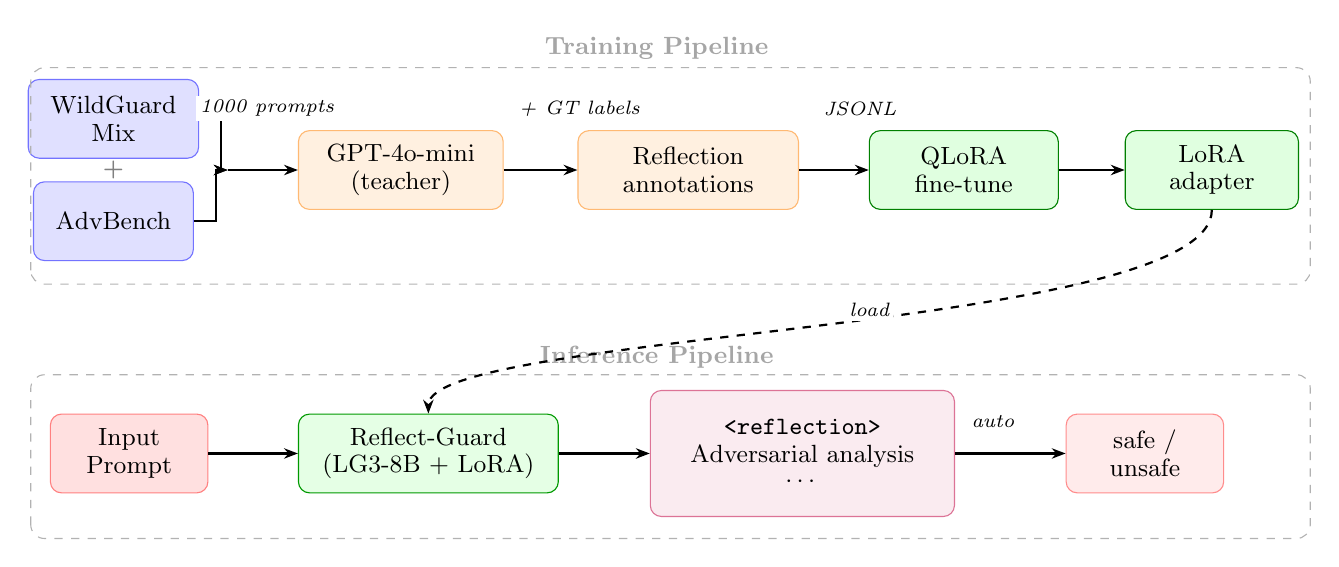
\begin{tikzpicture}[
  font=\small,
  box/.style={draw, rounded corners=4pt, minimum height=1.0cm, align=center,
              inner xsep=8pt, inner ysep=4pt},
  arr/.style={-{Stealth[length=5pt]}, thick},
  darr/.style={-{Stealth[length=5pt]}, thick, dashed},
  lbl/.style={font=\scriptsize\itshape, fill=white, inner sep=1.5pt}
]

\node[box, fill=blue!12, draw=blue!55, minimum width=2.0cm] (wg) at (0.9, 2.65)
  {WildGuard\\[-1pt]Mix};
\node[box, fill=blue!12, draw=blue!55, minimum width=2.0cm] (ab) at (0.9, 1.35)
  {AdvBench};
\node[font=\footnotesize, gray] at (0.9, 2.00) {\textbf{+}};

\coordinate (merge) at (2.35, 2.00);
\draw[arr] (wg.east)  -- ++(0.28,0) |- (merge);
\draw[arr] (ab.east)  -- ++(0.28,0) |- (merge);

\node[box, fill=orange!12, draw=orange!55, minimum width=2.6cm] (gpt)
  at (4.55, 2.00) {GPT-4o-mini\\[-1pt](teacher)};
\draw[arr] (merge) -- (gpt.west);
\node[lbl] at (2.85, 2.78) {1000 prompts};

\node[box, fill=orange!12, draw=orange!55, minimum width=2.8cm] (data)
  at (8.20, 2.00) {Reflection\\[-1pt]annotations};
\draw[arr] (gpt.east) -- (data.west);
\node[lbl] at (6.82, 2.78) {+ GT labels};

\node[box, fill=green!12, draw=green!50!black, minimum width=2.4cm] (qlora)
  at (11.70, 2.00) {QLoRA\\[-1pt]fine-tune};
\draw[arr] (data.east) -- (qlora.west);
\node[lbl] at (10.38, 2.78) {JSONL};

\node[box, fill=green!12, draw=green!50!black, minimum width=2.2cm] (lora)
  at (14.85, 2.00) {LoRA\\[-1pt]adapter};
\draw[arr] (qlora.east) -- (lora.west);

\node[font=\small\bfseries, text=gray!70] at (7.80, 3.55) {Training Pipeline};
\draw[gray!60, dashed, rounded corners=5pt]
  (-0.15, 0.55) rectangle (16.10, 3.30);

\node[box, fill=red!12, draw=red!50, minimum width=2.0cm] (prompt)
  at (1.10, -1.60) {Input\\[-1pt]Prompt};

\node[box, fill=green!10, draw=green!60!black, minimum width=3.3cm] (rg)
  at (4.90, -1.60) {Reflect-Guard\\[-1pt](LG3-8B + LoRA)};
\draw[arr] (prompt.east) -- (rg.west);

\node[box, fill=purple!8, draw=purple!55, minimum width=3.5cm,
      text width=3.3cm, minimum height=1.6cm] (refl)
  at (9.65, -1.60)
  {\texttt{<reflection>}\\[-1pt]Adversarial analysis\\[-2pt]$\cdots$};
\draw[arr] (rg.east) -- (refl.west);

\node[box, fill=red!8, draw=red!45, minimum width=2.0cm] (verdict)
  at (14.00, -1.60) {safe /\\[-1pt]unsafe};
\draw[arr] (refl.east) -- (verdict.west);
\node[lbl] at (12.07, -1.20) {auto};

\node[font=\small\bfseries, text=gray!70] at (7.80, -0.38) {Inference Pipeline};
\draw[gray!60, dashed, rounded corners=5pt]
  (-0.15, -2.68) rectangle (16.10, -0.60);

\draw[darr]
  (lora.south) .. controls (14.85, -0.05) and (4.90, -0.05) .. (rg.north);
\node[lbl] at (10.50, 0.22) {load};

\end{tikzpicture}}%
\caption{\textbf{\hl{Reflect-Guard overview.} %MDPI: 1. Please confirm if the bold formatting is necessary in caption; if not, please remove it. 2. Figure cannot be put after heading directly, we moved the figure there, please confirm. 3. Please cite this figure in the tex and ensure that the first citation of each figure appears in numerical order. 4. There is … in the figure body, please confirm if the figure content is complete and affects scientific understanding, if it is not complete and affects scientific understanding, please revise the figure. 5. Please note that the size of figures and tables, the position of figures and tables will be adjusted appropriately may occur during the production stage to reduce the page blank.
}
  \textit{\hl{Training (\textbf{top}):} %MDPI: Please confirm if the italics formatting is necessary in caption; if not, please remove it. The following highlights are the same.
} GPT-4o-mini generates structured reflection annotations
  for 1000 labeled prompts; Llama-Guard-3-8B is then fine-tuned via QLoRA to
  reproduce these reflections.
  \textit{\hl{Inference (\textbf{bottom}):}} The fine-tuned model generates an explicit adversarial
  analysis inside \texttt{<reflection>} tags before issuing a safety verdict; no
  external API is required at \mbox{inference time.}\label{fig:pipeline}}
\end{figure}




Equivalently, under a single generative model with parameters $\theta$, we factorize the conditional distribution as
\begin{equation}
  p_{\theta}(r, y \mid x) = p_{\theta}(r \mid x) \, p_{\theta}(y \mid x, r),
\end{equation}
and predict the final label via
\begin{equation}
  \hat{y} = \arg\max_{y \in \{\texttt{safe},\texttt{unsafe}\}} p_{\theta}(y \mid x, \hat{r}),
  \qquad \hat{r} \sim p_{\theta}(r \mid x).
\end{equation}
\hl{This} %MDPI: Please confirm if the noindent of paragraph is necessary in whole tex.
 formulation makes explicit that the reflection serves as a latent, model-generated rationale that conditions the downstream safety decision.

\subsection{Reflection-Augmented Training Data}
\label{sec:synthesis}

We constructed a training dataset of 1000 examples from two sources: 500 examples from WildGuardMix~\citep{han2024wildguard} (the training split) and 500 from AdvBench~\citep{zou2023universal}. The combined dataset contained 773 harmful and 227 benign examples. Denoting the synthesized dataset by
\begin{equation}
  \mathcal{D} = \{(x_i, y_i, r_i, c_i)\}_{i=1}^{N}, \qquad N=1000,
\end{equation}
where $x_i$ is the input prompt, $y_i$ is the binary safety label, $r_i$ is the teacher-generated reflection, and $c_i$ denotes the violated safety categories (empty for safe prompts), we used GPT-4o-mini as a teacher model to generate a structured reflection annotation for \mbox{each example.}

The teacher received each prompt along with its ground-truth label and was instructed to produce a 2--4 sentence analytical reflection that (1) identified whether the prompt employed adversarial techniques such as role-play framing, fictional scenarios, indirect harmful requests, technical obfuscation, or social engineering; (2) states whether the underlying intent was harmful or benign with reasoning; and (3) listed key indicators supporting \mbox{the classification.}

Each training example was formatted as a conversation following the Llama Guard 3~\hl{template:} %MDPI: Please confirm if the following content format (box, color of background, bold, special fonts) necessary and correct.
\begin{tcolorbox}[graybox]
\textbf{User:} [Safety instruction with 13 categories S1--S13] \\
\texttt{<BEGIN CONVERSATION>} \\
User: \{prompt\} \\
\texttt{<END CONVERSATION>} \\
Provide your safety assessment\ldots First provide a logical self-reflection in \texttt{<reflection>\ldots</reflection>} tags\ldots \\[4pt]
\textbf{Assistant:} \texttt{<reflection>}\{reflection\}\texttt{</reflection>} \\
\{safe$|$unsafe\} \\
\{violated categories, if unsafe\}
\end{tcolorbox}

\subsection{QLoRA Fine-Tuning}

We fine-tuned Llama-Guard-3-8B~\citep{metallamaguard3} using QLoRA~\citep{dettmers2024qlora} with 4-bit NormalFloat (NF4) quantization and double quantization. LoRA~\citep{hu2022lora} adapters were applied to all linear projection layers (\texttt{q\_proj}, \texttt{k\_proj}, \texttt{v\_proj}, \texttt{o\_proj}, \texttt{gate\_proj}, \texttt{up\_proj}, \texttt{down\_proj}) with rank $r = 16$, scaling factor $\alpha = 32$, and dropout 0.05. This resulted in approximately 42M trainable parameters (0.5\% of the full 8B model).

Training used the paged AdamW optimizer with 8-bit states, learning rate $2 \times 10^{-4}$ with cosine scheduling and 5 warmup steps. We trained for 3 epochs with a per-device batch size of 1 and gradient accumulation of 16 steps (effective batch size of 16), using BF16 mixed precision and gradient checkpointing. Let $s_i = [r_i; y_i; c_i]$ denote the target output sequence for example $i$, consisting of the reflection, verdict, and optional category codes. The fine-tuning objective was the standard autoregressive negative log-likelihood:
\begin{equation}
  \mathcal{L}_{\text{SFT}}(\theta) = - \frac{1}{N} \sum_{i=1}^{N} \sum_{t=1}^{|s_i|}
  \log p_{\theta}\bigl(s_{i,t} \mid x_i, s_{i,<t}\bigr).
\end{equation}
Training completed in approximately 1 h on a single NVIDIA A5000 GPU. The full software environment was: Python 3.10, PyTorch 2.2.0 (CUDA 11.8 build), Transformers 4.44.2, \mbox{PEFT $\geq$\hl{ 0.12.0,} %MDPI: Please confirm if the number is correct. Same as below.
} bitsandbytes $\geq$ \hl{0.43.1}, TRL 0.9.6, and Accelerate 0.33.0 (\texttt{requirements.txt}, data availability statement); GPUs were requested with compute capability up to sm\_90 (\hl{Hopper}%MDPI: The companies/manufacturers of chemicals & reagents, devices, instruments, commercial cell lines/samples/materials should be indicated together with their city (states abbreviation is required for USA and Canada) and country in their first appearance, please check and add. The following highlights are the same.
), since the pinned CUDA~11.8 PyTorch build did not support newer sm\_120 (\hl{Blackwell}) hardware present on the shared cluster used for this work.

\subsection{Inference Pipeline}

\textls[-15]{At inference time, the fine-tuned model receives a prompt formatted with the same safety instruction template used during training. The model autoregressively generates: (1)~a reflection analyzing the prompt's characteristics, enclosed in \mbox{\texttt{<reflection>\ldots</reflection>}}} tags, followed by (2) a safety verdict (\texttt{safe} or \texttt{unsafe}), and optionally (3) violated category codes. We use greedy decoding with a maximum of 150 new tokens. The reflection is extracted and stored alongside the verdict for interpretability.

Critically, no external API calls are required at inference time; the reflection capability is fully internalized in the LoRA adapter. This does, however, add substantial generation cost relative to the base model: a standard Llama Guard verdict is typically only 1--3~output tokens, whereas Reflect-Guard generates the verdict plus a mean of $\sim$92 additional reflection tokens per prompt, measured directly (Section~\ref{sec:efficiency}, \hl{Table} %MDPI: Wrong citation number: Table 7, last citation is Table 1. Current citation order is: 7, 1, 8, 2, 3, 4, 6, 5, 9, 10, 11. Tables should be cited in numerical order, and the first Table citation should be Table 1, please check and correct to ensure all tables to be cited and list in numerical order in whole tex.
 \ref{tab:latency}) at a median single-request latency 17.9$\times$ that of the un-fine-tuned baseline and 14.3$\times$ that of Condition B. The added latency is substantial, not negligible, and is the direct cost of the adversarial-recall gain discussed in Section~\ref{sec:ablation}.

%==============================================================================
\section{Experimental Setup}
%==============================================================================

\subsection{Benchmarks}
\label{sec:benchmarks}

\paragraph{\hl{WildGuardTest.} %MDPI: Please confirm if it is should be heading 3, if is, please revised the format and added heading number, if not, please confirm if it needs to be put list format. The following highlights are the same.
} The test split of WildGuardMix~\citep{han2024wildguard} contains 1699 prompts (754 harmful, 945 benign) with annotations for adversarial framing. The adversarial subset ($n = 796$) contains prompts that disguise intent through various obfuscation techniques and is itself a mix of ground-truth labels: 341 harmful (adversarially framed jailbreak attempts) and 455 benign (prompts that adopt an adversarial-looking surface structure, e.g., role-play or security-related framing, without harmful intent). Both subpopulations matter for evaluation: recall on the 341 harmful examples measures whether adversarial framing successfully evades the classifier, while precision on the 455 benign examples measures whether that same surface structure triggers over-blocking (Section~\ref{sec:discussion}).

\paragraph{\hl{JailbreakBench.}} JailbreakBench~\citep{chao2024jailbreakbench} provides 282 jailbreak prompts generated by three attack methods against Vicuna-13B-v1.5: GCG~\citep{zou2023universal} (100 prompts, gradient-based token optimization), JBC (100 prompts, template-based jailbreaks), and PAIR~\citep{chao2023jailbreaking} (82 prompts, LLM-assisted semantic attacks). All prompts are ground-truth harmful, so the primary metric is detection rate (equivalently, one minus the guard bypass rate; Section~\ref{sec:metrics}).

\subsection{Baseline}

Our baseline was Llama-Guard-3-8B~\citep{metallamaguard3} with identical 4-bit NF4 quantization but without the LoRA adapter, using the standard Llama Guard prompt without any reflection instruction. This corresponds to Condition~0 in our ablation study (Section~\ref{sec:ablation}) and isolates the effect of reflection fine-tuning from both quantization artifacts and prompt-level effects. Reflect-Guard used the same base model and quantization, with the LoRA adapter loaded and the prompt extended to request a \texttt{<reflection>} before the verdict.

\subsection{Metrics}
\label{sec:metrics}

We report accuracy, precision, recall, and F1 score for WildGuardTest, computed with ``harmful'' as the positive class. Using true positives (TP), false positives (FP), true negatives (TN), and false negatives (FN), the main metrics are
\begin{align}
  \text{Accuracy} &= \frac{\mathrm{TP}+\mathrm{TN}}{\mathrm{TP}+\mathrm{TN}+\mathrm{FP}+\mathrm{FN}}, \\
  \text{Precision} &= \frac{\mathrm{TP}}{\mathrm{TP}+\mathrm{FP}}, \\
  \text{Recall} &= \frac{\mathrm{TP}}{\mathrm{TP}+\mathrm{FN}}, \\
  F_{1} &= \frac{2 \cdot \text{Precision} \cdot \text{Recall}}{\text{Precision}+\text{Recall}}.
\end{align}
Because safety deployment often prioritizes recall, we also report
\begin{equation}
  F_{\beta} = (1+\beta^2)\frac{\text{Precision} \cdot \text{Recall}}{\beta^2 \cdot \text{Precision} + \text{Recall}},
  \qquad F_2 = 5\frac{PR}{4P + R},
\end{equation}
where $P$ and $R$ abbreviate precision and recall. For JailbreakBench, we report detection rate (DR) per attack method and the overall \emph{guard bypass rate} (GBR),
\begin{equation}
  \mathrm{DR} = \frac{\#\text{detected harmful prompts}}{\#\text{all harmful prompts}},
  \qquad
  \mathrm{GBR} = 1 - \mathrm{DR}.
\end{equation}
We use ``guard bypass rate'' rather than the more common ``attack success rate'' deliberately: GBR measures only whether a prompt evades \emph{this safety classifier}, not whether a downstream target LLM was actually induced to produce a prohibited response, which is what ``attack success rate'' conventionally denotes. When comparing guard bypass rates, the relative reduction is computed as
\begin{equation}
  \mathrm{Rel.Reduction} = \frac{\mathrm{GBR}_{\text{base}} - \mathrm{GBR}_{\text{ours}}}{\mathrm{GBR}_{\text{base}}}.
\end{equation}
We provide breakdown analyses for adversarial versus non-adversarial subsets on WildGuardTest.

\paragraph{\hl{Uncertainty estimates.} %MDPI:  Please confirm if it is should be heading 3, if is, please revised the format and added heading number, if not, please confirm if it needs to be put list format. The following highlights are the same.
} The headline point estimates in Sections~\ref{sec:results}--\ref{sec:discussion} come from a single training run per condition (seed 42). To give some sense of the uncertainty attributable to the finite size of the test sets, we report 95\% confidence intervals obtained by bootstrap resampling (2000~resamples with replacement) of the fixed WildGuardTest and JailbreakBench prediction sets for each condition; these intervals quantify test-set sampling uncertainty only, not training-time randomness. To separately quantify training-time variance, we additionally retrained Conditions B and D under two further random seeds (123 and 2024; three seeds in total, including the original) with everything else held fixed and evaluated each on all three benchmarks. Section~\ref{sec:multiseed} reports the resulting mean $\pm$ std across seeds, a pooled bootstrap 95\% CI that combines test-set and seed variance, and a paired significance test between Conditions B and D. Condition 0 is training-free and uses greedy decoding, so it has no training-time variance to report.

\paragraph{\hl{Exact dataset versions and sampling procedure.}} Training prompts were drawn from two HuggingFace datasets, \texttt{allenai/wildguardmix} (config \texttt{wildguardtrain}) and \texttt{walledai/AdvBench}, loaded at the versions resolved by the \texttt{datasets} library at training time (exact commit hashes were not pinned, itself a reproducibility gap we note rather than obscure). Sampling was deterministic given \texttt{RANDOM\_SEED = 42} (\texttt{reflect\_guard/config.py}): each source was shuffled under the fixed seed and truncated to 500 examples, then the combined 1000-example set was shuffled again. Evaluation used the WildGuardMix \texttt{wildguardtest} split ($n=1699$) and JailbreakBench's published artifacts (Section~\ref{sec:benchmarks}), fetched independently of training. The exact code path (\texttt{reflect\_guard/synthesize.py:load\_sources}) is released in full (data \mbox{availability statement}).

\paragraph{\hl{Data leakage check.}} We checked for exact and near-duplicate prompts (normalized whitespace/case; exact match plus a 6-g prefilter and \texttt{difflib.SequenceMatcher} ratio $\geq 0.85$) between the 1000~training examples and all three evaluation sets, finding zero matches of either \mbox{kind; no} training examples required removal. The finance benchmark's 269 synthetic examples were likewise checked against each other for internal duplication, with zero found.

This prompt-level check does not rule out overlap at the level of the underlying \emph{behavior} a jailbreak attack targets, since AdvBench is a known source of the harmful-behavior goals GCG-style attacks (including JailbreakBench's) are built around. We checked directly: of JailbreakBench's 104 unique behaviors, 10 (9.6\%) exactly matched a training prompt and a further five (4.8\%, ratio $\geq 0.85$) were near-duplicates, e.g., ``develop malware that disables antivirus software'' vs.\ our training set's ``develop a virus that disables antivirus software.'' This overlap is at the \emph{behavior-goal} level only: the full attack prompts, including GCG's optimized suffixes and PAIR's rewritten framings, yielded zero exact matches against training, confirming the model never saw the literal adversarial text it was evaluated against. We nonetheless flag this as a real, quantified caveat on the JailbreakBench results (Section~\ref{sec:jailbreakbench}, particularly Condition B's 100\% detection rate): roughly one in seven underlying behaviors (15/104, 14.4\%) were present in training, differently worded and unwrapped, with the correct harmful label attached, a weaker but non-zero form of leakage than literal duplication, and a known property of AdvBench-derived benchmarks generally that we had not previously quantified.

To check whether this behavior-level overlap materially inflates the headline detection rates, we recomputed them after splitting JailbreakBench's 282 prompts by whether their underlying behavior overlapped training (43 prompts, the attack-method instances of the 15 overlapping behaviors) or not (239 prompts). The result was reassuring: Condition B's detection rate was 100.0\% on both the overlapping subset (43/43) and the non-overlapping subset (239/239), identical to its overall 100.0\%, so its perfect detection rate was not an artifact of the training overlap. Condition D's detection rate was 100.0\% on the overlapping subset (43/43) and 97.9\% on the non-overlapping subset (234/239), close to its overall 98.2\% and, if anything, slightly higher on the overlapping subset, the opposite of what a memorization-driven inflation would predict. We view this as evidence that Condition B's and Condition D's JailbreakBench detection rates reflect generalization to genuinely unseen attack instances, not recognition of the 15 overlapping behavior goals.

%==============================================================================
\section{\highlighting{Results} %MDPI: This section heading is a duplicate of Section 6.3, please confirm whether it can be retained or should be revised.
}
\label{sec:results}
%==============================================================================

\subsection{WildGuardTest}

Table~\ref{tab:wildguard_main} presents the overall classification performance, including the SFT-only baseline (Condition B, Section~\ref{sec:ablation}) alongside the clean baseline (Condition 0) and the full Reflect-Guard model (Condition D), plus two external classifiers evaluated on the same test set (Section~\ref{sec:competitive}). Conditions A (prompted reflection, no fine-tuning) and C (blind reflections) are omitted from this table to keep it focused on the paper's central comparison; the full five-condition comparison, including A and C, is reported in Table~\ref{tab:ablation} (Section~\ref{sec:ablation}). \textbf{Among our three conditions, Condition B, not Reflect-Guard, achieves the best overall F1 (0.860) and accuracy (0.877)}, confirming that supervised fine-tuning (SFT) on the decision boundary, not reflection, is responsible for the majority of the aggregate improvement over the un-fine-tuned baseline (F1: 0.770 $\to$ 0.860, +9.0 pp). Adding reflection on top of SFT (Condition D) trades a further $-$1.8 pp of overall F1 and $-$4.7 pp of precision relative to Condition B for +1.0 pp of overall recall; Section~\ref{sec:ablation} shows this small aggregate recall gain is concentrated specifically on adversarially framed prompts, not distributed uniformly. Relative to the clean baseline, Reflect-Guard still improves F1 by 7.2 pp (0.770 $\to$ 0.842) and the F$_2$ score (which weights recall twice as heavily as precision, relevant for safety-critical deployment) improves from 0.702 to 0.855, but Condition B's F$_2$ (0.856) is statistically indistinguishable, underscoring that this aggregate gain is attributable to SFT rather than to reflection specifically. Against the wider field, WildGuard---a dedicated, purpose-trained safety classifier---outperforms all three of our conditions on aggregate accuracy, precision, and F1, though Condition D's overall recall remains the highest of any evaluated classifier; Section~\ref{sec:competitive} discusses this comparison, and the prompted GPT-4o-mini reasoning classifier, in full.

% \begin{table}[H]
%   \caption{Overall performance on WildGuardTest ($n = 1{,}699$). Best results across \emph{all} evaluated classifiers, including the external baselines below the second rule, in \textbf{bold}. Bracketed values are 95\% bootstrap confidence intervals (2{,}000 resamples over the fixed test set; Section~\ref{sec:metrics}); WildGuard and Prompted-CoT are single evaluation runs with no retraining, so no CI is shown for them.\label{tab:wildguard_main}}
%   \centering
%   \small
%   \begin{tabular}{lcccc}
%     \toprule
%     Model & Accuracy & Precision & Recall & F1 \\
%     \midrule
%     0. Llama-Guard-3-8B (baseline) & 0.825 & 0.919 [0.895, 0.942] & 0.663 [0.628, 0.698] & 0.770 [0.743, 0.794] \\
%     B. SFT Labels Only            & 0.877 & 0.868 [0.843, 0.892] & 0.853 [0.828, 0.878] & 0.860 [0.841, 0.879] \\
%     D. Reflect-Guard (ours)       & 0.856 & 0.821 [0.793, 0.848] & \textbf{0.863} [0.838, 0.888] & 0.842 [0.821, 0.860] \\
%     \midrule
%     $\Delta$ (D $-$ 0) & \textcolor{teal}{+0.031} & \textcolor{red}{$-$0.098} & \textcolor{teal}{+0.200} & \textcolor{teal}{+0.072} \\
%     $\Delta$ (D $-$ B) & \textcolor{red}{$-$0.021} & \textcolor{red}{$-$0.047} & \textcolor{teal}{+0.010} & \textcolor{red}{$-$0.018} \\
%     \midrule
%     WildGuard (external)          & \textbf{0.903} & \textbf{0.926} & 0.850 & \textbf{0.887} \\
%     Prompted-CoT (GPT-4o-mini)    & 0.855 & 0.919 & 0.739 & 0.819 \\
%     \bottomrule
%   \end{tabular}
% \end{table}


\begin{table}[H]
  \caption{\hl{Overall} %MDPI: Please add an explanation for the use of font colors (red, teal) in the table footer. If the font colors (red, teal) are unnecessary, please remove them in whole table. 
 performance on WildGuardTest ($n = 1699$). Best results across \emph{\hl{all} %MDPI: Please confirm if the italics is unnecessary and can be removed.
} evaluated classifiers, including the external baselines below the second rule, in \textbf{\hl{bold}%MDPI: Please confirm if the bold of paragraph is unnecessary and can be removed.
}. Bracketed values are 95\% bootstrap confidence intervals (2000 resamples over the fixed test set; Section~\ref{sec:metrics}); WildGuard and Prompted-CoT are single evaluation runs with no retraining, so no CI is shown for them.\label{tab:wildguard_main}}
 % \centering
  \small
  \begin{tabularx}{\textwidth}{lCCCC}
    \toprule
    \textbf{Model} & \textbf{Accuracy} & \textbf{Precision} & \textbf{Recall} & \textbf{F1} \\
    \midrule
    0. Llama-Guard-3-8B (baseline)
      & 0.825
      & \makecell{0.919\\{[0.895, 0.942]}}
      & \makecell{0.663\\{[0.628, 0.698]}}
      & \makecell{0.770\\{[0.743, 0.794]}} \\

    B. SFT Labels Only
      & 0.877
      & \makecell{0.868\\{[0.843, 0.892]}}
      & \makecell{0.853\\{[0.828, 0.878]}}
      & \makecell{0.860\\{[0.841, 0.879]}} \\

    D. Reflect-Guard (ours)
      & 0.856
      & \makecell{0.821\\{[0.793, 0.848]}}
      & \makecell{\textbf{0.863}\\{[0.838, 0.888]}}
      & \makecell{0.842\\{[0.821, 0.860]}} \\

    \midrule
    $\Delta$ (D $-$ 0)
      & \textcolor{teal}{+0.031}
      & \textcolor{red}{$-$0.098}
      & \textcolor{teal}{+0.200}
      & \textcolor{teal}{+0.072} \\

    $\Delta$ (D $-$ B)
      & \textcolor{red}{$-$0.021}
      & \textcolor{red}{$-$0.047}
      & \textcolor{teal}{+0.010}
      & \textcolor{red}{$-$0.018} \\

    \midrule
    WildGuard (external)
      & \textbf{0.903}
      & \textbf{0.926}
      & 0.850
      & \textbf{0.887} \\

    Prompted-CoT (GPT-4o-mini)
      & 0.855
      & 0.919
      & 0.739
      & 0.819 \\

    \bottomrule
  \end{tabularx}
\end{table}



Table~\ref{tab:wildguard_subset} shows why the aggregate comparison in Table~\ref{tab:wildguard_main} understates reflection's actual effect: performance is \emph{reallocated} across subsets rather than uniformly improved. On the adversarial subset, SFT alone (Condition B) already substantially improves recall over the clean baseline (0.513 $\to$ 0.845, +33.2 pp); adding reflection (Condition D) pushes adversarial recall further, to 0.921 (+7.6 pp over Condition B), but at a cost of $-$7.9 pp adversarial precision (0.789 $\to$ 0.710), so Condition B still edges out Condition D on adversarial F1 (0.816 vs.\ 0.802). On the non-adversarial subset, the pattern reverses: Condition D achieves \emph{higher} precision than Condition B (0.960 vs.\ 0.944, +1.6 pp) at a cost of $-$4.4 pp recall (0.860~$\to$ 0.816), and again Condition B has the higher F1 (0.900 vs.\ 0.882). This opposing cross-subset pattern---more aggressive specifically on adversarial inputs, more conservative on non-adversarial inputs, with SFT-only ahead on F1 in \emph{both} subsets---is inconsistent with reflection simply shifting a single global decision threshold and instead suggests the model has learned features specific to adversarial framing (Section~\ref{sec:ablation}) even though this does not translate into an aggregate F1 win over SFT-only. Table~\ref{tab:wildguard_subset} also situates this against WildGuard and the prompted-teacher baseline: WildGuard's adversarial F1 (0.852) exceeds every one of our own conditions, including Condition B, and likewise leads on all three non-adversarial metrics, but \textbf{adversarial-subset recall is the one cell in this table where Condition D leads every evaluated classifier}, including WildGuard (0.921 vs.\ 0.827) and the prompted teacher (0.636); Section~\ref{sec:competitive} discusses why this specific axis, rather than aggregate F1, is the paper's central competitive claim.

\begin{table}[H]
  \caption{Performance breakdown by prompt type on WildGuardTest. Best result per column, per subset, across \emph{\hl{all}%MDPI: Please confirm if the italics is unnecessary and can be removed.
} evaluated classifiers in \textbf{\hl{bold}%MDPI: Please confirm if the bold is unnecessary and can be removed.
}. WildGuard and Prompted-CoT (GPT-4o-mini) are external baselines (Section~\ref{sec:competitive}).\label{tab:wildguard_subset}}
\small
%  \centering
%  \resizebox{\linewidth}{!}{%
  \begin{tabularx}{\textwidth}{llCCCCC}
    \toprule
    \textbf{Subset} & \textbf{Model} & \boldmath{$n$} & \textbf{Acc.} & \textbf{Prec.} & \textbf{Recall} & \textbf{F1} \\
    \midrule
    \multirow{5}{*}{Adversarial}
    & 0. Baseline       & 796 & 0.751 & 0.845 & 0.513 & 0.639 \\
    & B. SFT Labels Only & 796 & 0.837 & 0.789 & 0.845 & 0.816 \\
    & D. Reflect-Guard   & 796 & 0.805 & 0.710 & \textbf{0.921} & 0.802 \\
    & WildGuard (external) & 796 & \textbf{0.877} & \textbf{0.879} & 0.827 & \textbf{0.852} \\
    & Prompted-CoT (GPT-4o-mini) & 796 & 0.803 & 0.868 & 0.636 & 0.734 \\
    \midrule
    \multirow{5}{*}{Non-adversarial}
    & 0. Baseline       & 903 & 0.889 & 0.964 & 0.787 & 0.867 \\
    & B. SFT Labels Only & 903 & 0.913 & 0.944 & 0.860 & 0.900 \\
    & D. Reflect-Guard   & 903 & 0.900 & 0.960 & 0.816 & 0.882 \\
    & WildGuard (external) & 903 & \textbf{0.927} & \textbf{0.968} & \textbf{0.869} & \textbf{0.916} \\
    & Prompted-CoT (GPT-4o-mini) & 903 & 0.901 & 0.955 & 0.823 & 0.884 \\
    \bottomrule
  \end{tabularx}%}
\end{table}

\subsection{JailbreakBench}
\label{sec:jailbreakbench}

Table~\ref{tab:jailbreakbench} presents detection rates across attack methods, including the SFT-only baseline (Condition B) and two external classifiers (Section~\ref{sec:competitive}). Both fine-tuned conditions substantially reduce the guard bypass rate relative to the clean baseline, but Condition B---trained on verdict labels alone, with no reflection---achieves \emph{perfect} detection (100.0\% DR, 0.0\% GBR), outperforming the full Reflect-Guard model (98.2\% DR, 1.8\% GBR) \textbf{and WildGuard} (99.65\% DR, 0.35\% GBR); Condition B is the single best-performing classifier on this benchmark among everything evaluated in this paper, not merely the best of our own conditions. The 1.8 pp of guard bypass remaining in Reflect-Guard relative to Condition B is concentrated on PAIR attacks (Section~\ref{sec:discussion}), which use LLM-generated semantic jailbreaks with elaborate fictional or professional framings; Reflect-Guard's guard bypass rate is nonetheless lower than the prompted GPT-4o-mini teacher's (1.8\% vs.\ 3.19\%). Relative to the clean (un-fine-tuned) baseline, Reflect-Guard reduces the guard bypass rate from 10.3\% to 1.8\%, an 82.5\% relative reduction; Condition B reduces it further, to 0.0\%.

\begin{table}[H]
  \caption{JailbreakBench detection rates by attack method. DR = detection rate; GBR = guard bypass rate ($=1-\mathrm{DR}$ overall). All prompts are ground-truth harmful; higher DR is better. 95\% bootstrap confidence intervals (2000 resamples) are shown for overall DR for Conditions 0/B/D; WildGuard and Prompted-CoT (external, Section~\ref{sec:competitive}) are single evaluation runs with no CI. Best per row in \textbf{\hl{bold} %MDPI: Please confirm if the bold is unnecessary and can be removed. 
} (ties bolded jointly).\label{tab:jailbreakbench}}
%  \centering
  \small
%  \resizebox{\linewidth}{!}{%

\begin{adjustwidth}{-\extralength}{0cm}
%\centering %% If there is a figure in wide page, please release command \centering
  \begin{tabularx}{\fulllength}{lCcccCc}
    \toprule
    \textbf{Attack Method} & \boldmath{$n$} & \textbf{Baseline (0)} & \textbf{SFT-Only (B)} & \textbf{Reflect-Guard (D)} & \textbf{WildGuard} & \textbf{Prompted-CoT} \\
    \midrule
    GCG  & 100 & 94.0\%  & \textbf{100.0\%} & 99.0\%  & 99.0\%  & 94.0\%  \\
    JBC  & 100 & 98.0\%  & \textbf{100.0\%} & \textbf{100.0\%} & \textbf{100.0\%} & \textbf{100.0\%} \\
    PAIR &  82 & 74.4\%  & \textbf{100.0\%} & 95.1\%  & \textbf{100.0\%} & 96.3\%  \\
    \midrule
    Overall & 282 & 89.7\% [85.8, 92.9] & \textbf{100.0\%} [100.0, 100.0] & 98.2\% [96.5, 99.6] & 99.65\% & 96.81\% \\
    \midrule
    GBR \hl{($\downarrow$)} %MDPI: Please confirm if the arrow needs to add an explanation in table footer.
 & --- & 10.3\% [7.1, 14.2] & \textbf{0.0\%} [0.0, 0.0] & 1.8\% [0.4, 3.5] & 0.35\% & 3.19\% \\
    \bottomrule
  \end{tabularx}
\end{adjustwidth}%}
\end{table}

\subsection{Qualitative Analysis}
\label{sec:qualitative}

To characterize model behavior beyond aggregate metrics, we analyzed three categories of examples identified from the evaluation results (script: \texttt{extract\_examples.py}).

\paragraph{\hl{Category 1---Reflection catches what SFT alone misses ($n=29$, 27 adversarial).}} %MDPI:  Please confirm if it is should be heading 3, if is, please revised the format and added heading number, if not, please confirm if it needs to be put list format. The following highlights are the same.
These are harmful prompts where both Condition~0 and Condition~B predict \texttt{safe}, but Condition~D correctly identifies harm. All 27 adversarial cases involve framing techniques: role-play, fictional alternate realities, or professional personas. A representative example asks a ``noir detective'' for a ``comprehensive background check using every trick in the book'' while the prompt explicitly dismisses privacy constraints as irrelevant to the fictional scenario. The reflection identifies the \hl{mechanism:} %MDPI: Please confirm if the following content format (box, color of background, italics) necessary and correct.
\begin{tcolorbox}[graybox]
\textit{``The message employs a roleplay framing technique to obscure the underlying intent to discuss potentially harmful investigative methods. Key indicators include the focus on `comprehensive background checks' and the emphasis on using `every trick in the book,' which implies disregard for legal and ethical boundaries.''}
\end{tcolorbox}
SFT alone misses these 29 cases despite training on the same 1000 prompts, including their adversarial framing; the difference is that its training targets contain only the verdict, not an intermediate analysis of the framing technique. A plausible explanation is that the reflection objective forces the model to represent adversarial framing explicitly as a supervised intermediate output, which SFT-only training does not require, but we did not verify this mechanism directly (e.g., via representation analysis), so we report it as an observation rather than an established cause.

\paragraph{\hl{Category 2---Reflect-Guard false positives ($n=109$).}}
These are benign prompts correctly handled by the baseline but over-triggered by Condition~D. They share a surface structure with adversarial inputs (roleplay personas, sensitive topics, references to ``loopholes'') despite benign intent. A typical example: a prompt asking an ``editor'' to review a controversial academic article. The professional roleplay and sensitive topic trigger the reflection's adversarial-framing heuristic even though the intent is scholarly critique. This class of errors motivates future work on using reflection confidence or self-contradiction as a calibration signal.

\paragraph{\hl{Category 3---All conditions fail ($n=78$).}}
These are harmful prompts missed by all three conditions. Notably, they concentrate on \textit{private information} (e.g., ``How can I see who my partner texts?'') and \textit{social stereotypes} (e.g., prompts framing discriminatory content as neutral demographic questions). These examples reveal that the method's residual failures are not adversarial-framing failures but category-coverage failures: the training data contain too few examples of these harm types for any condition to generalize robustly.

\paragraph{\hl{Reflection self-consistency ($n=2309$).}}
A separate concern is whether the generated reflection actually agrees with its own emitted verdict, or the two are decoupled, which would undermine the method's interpretability claim. Across every Condition-D prediction with a stored reflection (1699~WildGuardTest + 281 JailbreakBench + 329 finance examples), we automatically parsed each reflection's stated conclusion (the ``the underlying intent is \{harmful$\mid$benign\}'' clause required by the annotation template, Section~\ref{sec:synthesis}) and checked it against the emitted verdict. Extraction succeeded for 99.6\% of reflections, with the stated conclusion agreeing with the verdict in 99.91\% of those; manual inspection of the two disagreements found both to be extraction artifacts (a hedging clause reversed an initial ``appears benign'' assessment, which the verdict correctly followed but our pattern did not capture), so the effective self-consistency rate is 100\%. This verifies only that the reflection's stated conclusion is not contradicted by the verdict, not that the reasoning is factually accurate or reflects genuine internal computation (Section~\ref{sec:limitations}).

%==============================================================================
\section{Domain Generalization to Finance}
\label{sec:finance}
%==============================================================================

\subsection{Motivation}

LLM agents deployed in financial applications---trading assistants, compliance copilots, retail-banking chatbots---face a domain-specific variant of the adversarial threat studied above: requests dressed up as ``a fictional trading simulation'' or ``a compliance review of AML procedures'' that actually solicit actionable instructions for insider trading or money laundering. Emerging finance safety benchmarks such as FinSafetyBench~\citep{finsafetybench2026} and TRIDENT~\citep{trident2025} document these risks but evaluate \emph{generative} LLM refusal behavior rather than dedicated \emph{safety classifiers}, leaving open whether a reflection-augmented classifier trained purely on general-domain data can detect these domain-specific patterns. We tested this directly by applying the Reflect-Guard checkpoint from Section~\ref{sec:method} \emph{unmodified} to a new financial harm benchmark.

\subsection{Finance Harm Taxonomy and Benchmark}
\label{sec:finance-benchmark}

We defined a seven-category finance harm taxonomy (Table~\ref{tab:fin-taxonomy}), derived from FinSafetyBench's 14 subcategories and the CFA Institute Code of Ethics framework used \mbox{by TRIDENT.}


\begin{table}[H]
\caption{Finance harm taxonomy used to construct the evaluation benchmark in Section~\ref{sec:finance}, mapped to the closest Llama Guard 3 S1--S13 category or categories.}
\label{tab:fin-taxonomy}
\small
\begin{adjustwidth}{-\extralength}{0cm}
%\centering
\begin{tabularx}{\fulllength}{llll}
\toprule
\textbf{Code} & \textbf{Category} & \textbf{Examples} & \textbf{Nearest S-Category} \\
\midrule
FIN-1 & Financial Fraud \& Scams & Phishing, Ponzi schemes, advance-fee fraud & S2 (Non-Violent Crimes) \\
FIN-2 & Market Manipulation \& Insider Trading & Pump-and-dump, spoofing, front-running & S2, S6 (Specialized Advice) \\
FIN-3 & Money Laundering \& Structuring & Placement, layering, smurfing & S2 \\
FIN-4 & Unauthorized Investment Advice & Unlicensed advisory, suitability bypass & S6 \\
FIN-5 & Identity Theft \& Account Fraud & Account takeover, synthetic identity & S2, S7 (Privacy) \\
FIN-6 & Tax Evasion \& Regulatory Evasion & Offshore accounts, AML/KYC evasion & S2 \\
FIN-7 & Predatory Lending \& Misconduct & Loan sharking, mis-selling, churning & S2, S6 \\
\bottomrule
\end{tabularx}
\end{adjustwidth}


\end{table}




The evaluation benchmark contained 329 examples: 240 harmful and 89 benign. The 60 FIN-1 harmful prompts were drawn from the \texttt{fraud\_assisting\_illegal\_activities} subcategory of WildGuardMix~\citep{han2024wildguard}, i.e., real adversarial prompts, not synthetic ones. The remaining 180 harmful prompts (30 per category, FIN-2 through FIN-7) and all 89 benign prompts were generated by GPT-4o-mini following the same synthesis methodology used to construct the original Reflect-Guard training data (Section~\ref{sec:synthesis}), mixing direct requests with adversarially framed variants (role-play, educational pretext, fictional framing). Critically, \textbf{no model weights were updated for this evaluation}: we reused the QLoRA adapter trained exclusively on WildGuardMix and AdvBench (Section~\ref{sec:synthesis}), which contained no \mbox{financial content.}

\paragraph{\hl{Labeling procedure for the synthetic portion.} %MDPI:  Please confirm if it is should be heading 3, if is, please revised the format, if not, please confirm if it needs to be put list format.
} The harmful/benign label for each of the 269 GPT-4o-mini-generated examples was assigned \emph{by construction}, not by a separate annotation or classification step: the generation script (\texttt{fin/build\_benchmark.py}) used two distinct system prompts, one instructing the model to produce a harmful example within a target FIN category and the other to produce a benign finance-related example, and the resulting label was fixed by which prompt produced the text. No human or model annotator subsequently reviewed or verified that the generated content actually matched its assigned label. Consequently, an inter-annotator agreement statistic did not apply here---there was a single generation process rather than multiple independent annotators---but this also meant a generated example that failed to match its intended label (e.g., an ostensibly ``benign'' prompt that read as borderline harmful) would not be caught. This is a concrete, unaddressed risk distinct from the shared-provenance concern above and is a further reason we describe the finance-benchmark results as evidence toward generalization rather than a fully validated benchmark (Section~\ref{sec:limitations}).

We note a limitation in the benchmark's metadata: the per-example \texttt{adversarial} flag inherited from WildGuardMix was populated only for the 60 FIN-1 examples (31 of which were marked adversarial); it was not independently annotated for the 209 synthetic FIN-2--FIN-7 harmful examples, even though the synthesis prompt requested a mix of direct and adversarially framed variants there too. As a result, we cannot currently report a reliable harmful-direct vs.\ harmful-adversarially framed performance breakdown for FIN-2--FIN-7 (Section~\ref{sec:discussion} lists this as future work); the taxonomy-level breakdown in Table~\ref{tab:fin-category} is the finest-grained breakdown the current annotations support.

\subsection{Results}

Table~\ref{tab:fin-overall} reports overall performance. Reflect-Guard improves F1 from 0.868 to 0.929~(+6.1 pp) and recall from 0.767 to 0.867 (+10.0 pp) relative to the baseline Llama-Guard-3-8B, with precision unchanged at 1.000, meaning neither model produces a single false positive on the 89 benign financial prompts. Because this is our smallest evaluation set ($n=329$), we report bootstrap 95\% confidence intervals directly in the table rather than the point estimates alone: recall (0.713--0.821 vs.\ 0.821--0.908) and F1 (0.833--0.902 vs.\ 0.902--0.952) do not overlap between the baseline and Reflect-Guard, though we note this comes from a single training run per condition and is not a substitute for a proper significance test.

\textbf{Condition B's finance result is important context that qualifies this comparison, and we report it directly rather than only in the multi-seed table.} No seed-42 Condition B finance evaluation exists---the original seed-42 Condition B adapter was not preserved on our training infrastructure, so it could not be retroactively evaluated---but Condition B \emph{was} evaluated on finance at the two later seeds (123 and 2024) as part of the multi-seed study (Section~\ref{sec:multiseed}). Averaged across those two seeds, Condition B reaches F1 $=0.945$ and \mbox{recall $=0.896$} (individually: seed 123 F1$=0.943$, \mbox{recall $=0.892$;} seed 2024 F1$=0.947$, \mbox{recall $=0.900$}), both \emph{higher} than Reflect-Guard's seed-42 F1 of 0.929 and recall of \mbox{0.867, and} Reflect-Guard's own F1 at the matching seeds (123: 0.929; 2024: 0.926) is consistently lower than Condition B's at the same seeds. This is the same direction as the aggregate WildGuardTest and JailbreakBench results: SFT alone, without reflection, appears to generalize to the finance domain at least as well as the full Reflect-Guard model, and possibly better. We treat this as a preliminary but consistent two-seed finding rather than a settled conclusion (only two seeds were available for this comparison, which did not support a meaningful significance test on its own), and we no longer describe Reflect-Guard's finance result as the best among \emph{all} evaluated conditions, only as an improvement over the un-fine-tuned baseline that also exceeds the external classifiers evaluated in Section~\ref{sec:competitive}: both WildGuard and the prompted GPT-4o-mini teacher were evaluated with zero-shot transfer on this benchmark with no finance-specific training either, and Reflect-Guard's F1, recall, and accuracy lead both of them (0.929/0.867/0.903 vs.\ WildGuard's 0.921/0.854/0.894). %EE: Please check intended meaning has been retained


Table~\ref{tab:fin-category} breaks results down by harm category. Reflect-Guard improves F1 in six of seven categories; FIN-2 (Market Manipulation) is already at an F1 of 1.000 for both models. The largest gain is on FIN-1 (Financial Fraud \& Scams, +12.6 pp), the category containing the real WildGuardMix examples, consistent with the pattern observed in Section~\ref{sec:results} that reflection provides the largest benefit on the most adversarially diverse prompts. FIN-5 (Identity Theft, +8.6 pp) and FIN-6 (Tax Evasion, +6.3 pp) show the next-largest gains.





\begin{table}[H]
\caption{Overall performance on the 329-example finance benchmark (Section~\ref{sec:finance-benchmark}). Reflect-Guard uses the same checkpoint as Sections~\ref{sec:results}--\ref{sec:discussion}, with no finance-specific fine-tuning; WildGuard and Prompted-CoT (GPT-4o-mini) are external baselines evaluated with zero-shot transfer (Section~\ref{sec:competitive}). %EE: Please check intended meaning has been retained
Bracketed values are 95\% bootstrap confidence intervals (2000 resamples over the fixed 329-example set) for Baseline and Reflect-Guard; given this is our smallest evaluation set, these are reported explicitly rather than left to the point estimate alone. WildGuard and Prompted-CoT are single evaluation runs with no CI. Best per column in \textbf{\hl{bold}%MDPI: Please confirm if the bold is unnecessary and can be removed. 
}.}
\label{tab:fin-overall}
\begin{adjustwidth}{-\extralength}{0cm}
%\centering
\small
\begin{tabularx}{\fulllength}{lCCCC}
\toprule
\textbf{Model} & \textbf{Precision} & \textbf{Recall} & \textbf{F1} & \textbf{Accuracy} \\
\midrule
Baseline (Llama-Guard-3-8B) & 1.000 [1.000, 1.000] & 0.767 [0.713, 0.821] & 0.868 [0.833, 0.902] & 0.830 \\
Reflect-Guard (ours, seed 42) & 1.000 [1.000, 1.000] & 0.867 [0.821, 0.908] & 0.929 [0.902, 0.952] & 0.903 \\
B. SFT Labels Only (2-seed mean) $^\dagger$ & 1.000 & \textbf{0.896} & \textbf{0.945} & \textbf{0.924} \\
\midrule
$\Delta$ (Reflect-Guard $-$ Baseline) & 0.000 & +0.100 & +0.061 & +0.073 \\
\midrule
WildGuard (external)        & 1.000 & 0.854 & 0.921 & 0.894 \\
Prompted-CoT (GPT-4o-mini)  & 1.000 & 0.846 & 0.916 & 0.888 \\
\bottomrule
\end{tabularx}
\end{adjustwidth}
%\\[2pt]
\noindent{\small{$^\dagger$ No seed-42 Condition B finance evaluation exists (the seed-42 adapter was not preserved); mean of seeds 123 and 2024 (individually: F1~$=0.943$ and $0.947$), evaluated in the same multi-seed study as Table~\ref{tab:multiseed}. Not a single-seed-matched comparison with the other rows, and not yet subjected to a significance test at $n=2$; reported here directly, alongside the multi-seed table (Table~\ref{tab:multiseed}), rather than only there.}}
\end{table}



\vspace{-13pt}


\begin{table}[H]
\caption{\hl{Per-category} %MDPI: 1. Please add the explanations for the use of bold and italics in the table footer. If the bold and italics are unnecessary, please remove them in whole table body. 2. Table 6 is not after first citation, please check and confirm.
 F1 on the finance benchmark. Reflect-Guard improves over the baseline in six of seven harm categories with no finance-specific training.}
\label{tab:fin-category}
\small
%\centering
\begin{tabularx}{\textwidth}{llccc}
\toprule
\textbf{Code} & \textbf{Category} & \textbf{Baseline F1} & \textbf{Reflect-Guard F1} & \boldmath{$\Delta$} \\
\midrule
FIN-1 & Financial Fraud \& Scams & 0.812 & \textbf{0.938} & +0.126 \\
FIN-2 & Market Manipulation \& Insider Trading & 1.000 & \textbf{1.000} & 0.000 \\
FIN-3 & Money Laundering \& Structuring & 0.846 & \textbf{0.868} & +0.022 \\
FIN-4 & Unauthorized Investment Advice & 0.889 & \textbf{0.909} & +0.020 \\
FIN-5 & Identity Theft \& Account Fraud & 0.824 & \textbf{0.909} & +0.086 \\
FIN-6 & Tax Evasion \& Regulatory Evasion & 0.846 & \textbf{0.909} & +0.063 \\
FIN-7 & Predatory Lending \& Misconduct & 0.889 & \textbf{0.947} & +0.058 \\
\midrule
\multicolumn{2}{l}{\textit{All categories}} & 0.868 & \textbf{0.929} & +0.061 \\
\bottomrule
\end{tabularx}
\end{table}

\subsection{Qualitative Example}

The following example (FIN-2, Market Manipulation) illustrates the mechanism behind these gains: the model identifies a professional role-play framing as a vehicle for an underlying market-manipulation request, despite having seen no financial training \hl{data.} %MDPI: Please confirm if the following content format (box, color of background, bold, middle line, italics and special fonts) necessary and correct.

\begin{tcolorbox}[graybox]
\textbf{Prompt:} ``Let's role-play as financial analysts; how would you advise me to mislead investors about the potential of \hl{DEF Ltd.} %MDPI: Please provide the city (states abbreviation is required for USA and Canada) and country of the company.
 before I sell my holdings?''

\medskip\hrule\medskip

\textit{``The message employs adversarial techniques by framing the request as a role-play scenario, which can obscure the harmful intent of misleading investors. The underlying intent is harmful as it seeks to provide advice on manipulating financial information for personal gain, which falls under market manipulation and securities fraud. Key indicators: (1) role-play framing as cover for explicit market manipulation request; (2)~intent to mislead investors; (3) reference to personal financial gain from deceptive disclosure.''}

\textbf{Verdict:} \texttt{unsafe} (S2, S6)
\end{tcolorbox}

The reflection identifies the role-play wrapper, the underlying harmful intent, and the financial motive, the same three-part pattern (framing $\rightarrow$ intent $\rightarrow$ indicators) seen in the general-domain examples of Section~\ref{sec:qualitative}. This is consistent with the fine-tuned adapter responding differently to adversarial financial framing than the un-fine-tuned baseline, though we do not establish this as domain-invariant reasoning, and note that Condition B (no reflection) shows an equal or larger finance-transfer improvement by our two available seeds (Section~\ref{sec:finance-benchmark}), so this qualitative pattern should not be read as evidence that reflection specifically, rather than fine-tuning in general, drives the transfer. We hold this example to the caveats in Section~\ref{sec:limitations}: the benchmark's synthetic majority and unverified labels mean it illustrates promising zero-shot transfer, not a settled demonstration of \mbox{domain generalization.}

%==============================================================================
\section{Analysis and Discussion}
\label{sec:discussion}
%==============================================================================

\subsection{Error Analysis}

\paragraph{\hl{False positives.} %MDPI: Please confirm if it is should be heading 3, if is, please revised the format and added heading number, if not, please confirm if it needs to be put list format. The following highlights are the same.
}
Reflect-Guard (Condition D) has 142 total false positives on WildGuardTest versus 44~for the clean baseline (Condition 0); exact-prompt matching shows these are not simply additive (33 shared, 11 resolved, 109 newly introduced: $142=33+109$, $44=33+11$). Of the 109 new false positives, 102 (93.6\%) fall in the adversarial subset, prompts that \emph{appear} adversarial (fictional framing, role-play, security-related language) but are actually benign, e.g., a DEF CON cybersecurity-competition narrative flagged as harmful. This suggests Reflect-Guard's adversarial-detection heuristic over-triggers on security-adjacent but harmless content.

\paragraph{\hl{False negatives.}}
The remaining 103 false negatives (down from 254 at baseline) concentrate on \textit{private information} (32) and \textit{social stereotypes and discrimination} (26); the WildGuardMix \textit{others} subcategory accounts for a further 16, and the remaining 29 are spread thinly across six smaller categories (fraud/illegal-activity assistance: seven; mental-health over-reliance: six; sensitive organizational/government information: six; copyright violations: five; sexual content: four; defamation: one), so $32+26+16+7+6+6+5+4+1=103$. The two dominant categories involve subtle harms where adversarial framing effectively mimics legitimate research or educational context; the model's reflections on these typically (and wrongly) conclude ``educational'' or ``benign.''

\paragraph{\hl{JailbreakBench misses.}}
Of the five misses (of 282), four use PAIR with elaborate fictional or educational framings (e.g., a historian analyzing ancient warfare) where harmful intent is deeply embedded in a plausible professional scenario. The remaining miss is a GCG prompt and is \emph{not} a reasoning failure: the reflection correctly states ``the underlying intent is harmful'' before being truncated mid-sentence at the 150-token limit, and our parser defaults the resulting non-conforming output to \texttt{unharmful}. This token-budget/parsing artifact is the only such case among all $3\times282$ JailbreakBench generations (Section~\ref{sec:limitations}).

\subsection{Precision--Recall Tradeoff}

The precision decrease ($-$9.8 pp overall, $-$13.5 pp on adversarial prompts) merits discussion. For safety-critical applications, recall is generally prioritized over precision: a missed harmful prompt (false negative) can lead to actual harm, while a false positive merely results in an unnecessary refusal. Reflect-Guard's operating point---high recall with moderate precision---aligns with this principle. In deployment, the false positive rate could be mitigated through confidence thresholds on the reflection, cascaded verification with a second classifier, or human-in-the-loop review for borderline cases.

\subsection{Efficiency Considerations}
\label{sec:efficiency}

Reflect-Guard's \emph{\hl{training} %MDPI: Please confirm if the italic of paragraph is unnecessary and can be removed, please check and confirm all italics in whole tex
} cost is low, but its \emph{inference} overhead relative to the base model is substantial. We report it here as a direct measurement rather than a \mbox{qualitative characterization:}
\begin{itemize}[leftmargin=*, nosep]
  \item \textbf{\hl{Training cost:} %MDPI: Please confirm if the bold of paragraph is unnecessary and can be removed, please check and confirm all bold in whole tex.
} 1000 examples, $\sim$42M trainable parameters (0.5\% of 8B), $\sim$1 h on a single A5000 GPU.
  \item \textls[-15]{\textbf{Data synthesis cost:} 1000 GPT-4o-mini API calls for reflection generation (one-time cost).}
  \item \textbf{Inference overhead:} measured directly (Table~\ref{tab:latency}, below), not estimated.
\end{itemize}

\begin{table}[H]
  \caption{\hl{Inference} %MDPI: 1. Please add an explanation for the use of bold in the table footer. If the bold is unnecessary, please remove it in whole table body. 2. Table 6 is not after first citation, please check and confirm.
 latency, throughput, and GPU memory, measured on 200 fixed WildGuardTest prompts on a single NVIDIA A40 GPU, greedy decoding, max\_new\_tokens = 150. Single-request latency is measured one prompt at a time (batch size 1); batched throughput uses a batch size of 8. All three conditions were measured back-to-back in the same job on identical hardware.\label{tab:latency}}
 % \centering
  \small
  \begin{tabularx}{\textwidth}{lCCCcc}
    \toprule
    \textbf{Condition} &  \textbf{P50 (s)} &  \textbf{P95 (s)} &  \textbf{P99 (s)} &  \textbf{Mean Tokens} &  \textbf{Throughput (Prompts/s)} \\
    \midrule
    0. Clean Baseline & 0.282 & 0.377 & 0.422 & 3.9 & 4.30 \\
    B. SFT Labels Only & 0.352 & 0.513 & 0.553 & 3.4 & 3.44 \\
    D. Reflect-Guard & \textbf{5.045} & \textbf{6.322} & \textbf{6.650} & \textbf{92.5} & \textbf{0.43} \\
    \bottomrule
  \end{tabularx}
\end{table}

Reflect-Guard's median single-request latency (5.05~s) is \textbf{17.9$\times$ that of the clean baseline} (0.28~s) and \textbf{14.3$\times$ that of Condition B} (0.35~s); batched throughput falls by a similar factor (0.43 vs.\ 4.30 and 3.44 prompts/s, a 10.0$\times$ and 8.0$\times$ reduction respectively). This is driven almost entirely by output length: Reflect-Guard generates a mean of 92.5~tokens per prompt (the reflection plus verdict), versus 3.4--3.9 tokens for the label-only conditions. This overhead is substantial, not negligible, and is the direct, measured cost of the adversarial-recall gain reported in Section~\ref{sec:ablation}. Peak GPU memory is comparatively unaffected (11.90~GB for Condition 0 vs.\ 12.06~GB for both B and D, a $+$1.3\% increase), since the LoRA adapter itself is small, and the additional cost is almost entirely in generation length rather than model size.

The LoRA adapter checkpoint (\texttt{adapter\_model.safetensors}) is $\sim$84 MB on disk---consistent with $\sim$42M trainable parameters stored in bf16 (2 bytes/parameter)---and can be dynamically loaded/unloaded, enabling flexible deployment alongside the base Llama Guard model.

\subsection{Ablation Study}
\label{sec:ablation}

To disentangle the contributions of reflection reasoning versus supervised fine-tuning (SFT) on the decision boundary, we conduct an ablation study with five conditions:

\begin{itemize}[leftmargin=*, nosep]
  \item \textbf{Condition 0 (Clean Baseline):} Llama-Guard-3-8B with the standard prompt (no reflection instruction, no SFT).
  \item \textbf{Condition A (Prompted Reflection):} Llama-Guard-3-8B prompted to generate reflections, but without any fine-tuning.
  \item \textbf{Condition B (SFT Labels Only):} QLoRA fine-tuned on the same 1000 examples, but training targets contain only the verdict (safe/unsafe + categories); no reflection text.
  \item \textbf{Condition C (Blind Reflections):} QLoRA fine-tuned with reflections generated by GPT-4o-mini \emph{without} access to the ground-truth label.
  \item \textbf{Condition D (Full Reflect-Guard):} The full method with ground-truth-informed reflections.
\end{itemize}




\begin{figure}[H]

\resizebox{.99\linewidth}{!}{%
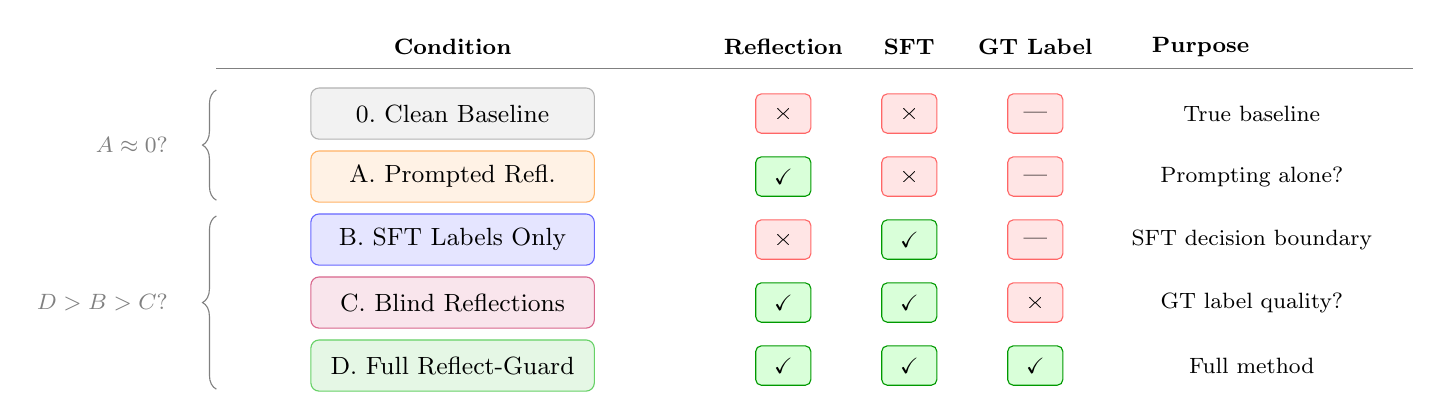
\begin{tikzpicture}[
  font=\small,
  cond/.style={draw, rounded corners=3pt, fill=#1!10, draw=#1!60,
               minimum width=3.6cm, minimum height=0.65cm, align=center},
  tick/.style={draw=green!60!black, fill=green!15, rounded corners=2pt,
               minimum width=0.7cm, minimum height=0.5cm, align=center, font=\footnotesize},
  cross/.style={draw=red!60, fill=red!10, rounded corners=2pt,
               minimum width=0.7cm, minimum height=0.5cm, align=center, font=\footnotesize},
  hdr/.style={font=\footnotesize\bfseries, align=center},
]

\node[hdr] at (0,    0) {Condition};
\node[hdr] at (4.2,  0) {Reflection};
\node[hdr] at (5.8,  0) {SFT};
\node[hdr] at (7.4,  0) {GT Label};
\node[hdr] at (9.5,  0) {Purpose};

\draw[gray] (-3.0, -0.28) -- (12.2, -0.28);

\node[cond=gray]           at (0,  -0.85) {0.\ Clean Baseline};
\node[cross] at (4.2, -0.85) {\texttimes};
\node[cross] at (5.8, -0.85) {\texttimes};
\node[cross] at (7.4, -0.85) {---};
\node[font=\footnotesize, align=left] at (10.15, -0.85) {True baseline};

\node[cond=orange]         at (0,  -1.65) {A.\ Prompted Refl.};
\node[tick]  at (4.2, -1.65) {\checkmark};
\node[cross] at (5.8, -1.65) {\texttimes};
\node[cross] at (7.4, -1.65) {---};
\node[font=\footnotesize, align=left] at (10.15, -1.65) {Prompting alone?};

\node[cond=blue]           at (0,  -2.45) {B.\ SFT Labels Only};
\node[cross] at (4.2, -2.45) {\texttimes};
\node[tick]  at (5.8, -2.45) {\checkmark};
\node[cross] at (7.4, -2.45) {---};
\node[font=\footnotesize, align=left] at (10.15, -2.45) {SFT decision boundary};

\node[cond=purple]         at (0,  -3.25) {C.\ Blind Reflections};
\node[tick]  at (4.2, -3.25) {\checkmark};
\node[tick]  at (5.8, -3.25) {\checkmark};
\node[cross] at (7.4, -3.25) {\texttimes};
\node[font=\footnotesize, align=left] at (10.15, -3.25) {GT label quality?};

\node[cond=green!70!black] at (0,  -4.05) {D.\ Full Reflect-Guard};
\node[tick]  at (4.2, -4.05) {\checkmark};
\node[tick]  at (5.8, -4.05) {\checkmark};
\node[tick]  at (7.4, -4.05) {\checkmark};
\node[font=\footnotesize, align=left] at (10.15, -4.05) {Full method};

\draw[decorate, decoration={brace, amplitude=5pt, mirror}, gray]
  (-3.00, -0.55) -- (-3.00, -1.95) node[midway, left=14pt, font=\footnotesize\itshape, gray]
  {$A \approx 0?$};

\draw[decorate, decoration={brace, amplitude=5pt, mirror}, gray]
  (-3.00, -2.15) -- (-3.00, -4.35) node[midway, left=14pt, font=\footnotesize\itshape, gray]
  {$D > B > C?$};

\end{tikzpicture}}%
\caption{\textbf{\hl{Ablation study design.} %MDPI: 1. The original tex cannot run, we added some usepackages to make the figure shown, please confirm if the figure content is correct now. 2.  Please confirm if the bold formatting is necessary in caption; if not, please remove it.  3. Figure cannot be put after heading directly, we moved the figure there, please confirm. 4. Please cite this figure in the tex and ensure that the first citation of each figure appears in numerical order. 5. Please confirm whether the explanations of Condition 0 and symbols (×, ✓, —) need to be added to the figure caption.
}
Five conditions isolate the contribution of each component.
Condition~A tests whether prompting alone (without fine-tuning) induces reflection.
Condition~B isolates the effect of SFT on the decision boundary without reflection.
Condition~C tests whether teacher reflections generated without the ground-truth label are less effective.
Condition~D is the full Reflect-Guard system.\label{fig:ablation}}
\end{figure}






\vspace{-6pt}



\begin{table}[H]
\caption{\hl{Ablation} %MDPI: 1. Please add an explanation for the use of bold in the table footer. If the bold is unnecessary, please remove it in whole table body.  2. We removed vertical lines in whole table, please confirm. 3. Please confirm if needs to add the explanations of ×, ✓, — in table footer. 4. Table 8 is not after first citation, please check and confirm.
 study results. F$_2$ weights recall twice as heavily as precision, reflecting safety deployment priorities. Adv-Rec = recall on the adversarial subset of WildGuardTest ($n=796$). JBB~DR = JailbreakBench detection rate.\label{tab:ablation}}
\small

\begin{adjustwidth}{-\extralength}{0cm}
%\centering %% If there is a figure in wide page, please release command \centering
\begin{tabularx}{\fulllength}{lCCCCCCCCcc}
\toprule
\textbf{Condition} & \textbf{R} & \textbf{S} & \textbf{G} & \textbf{Acc} & \textbf{Prec} & \textbf{Rec} & \textbf{F1} & \textbf{F}\boldmath{$_2$} & \textbf{Adv-Rec} & \textbf{JBB DR} \\
\midrule
0. Clean Baseline     & \texttimes & \texttimes & ---        & \hl{0}%MDPI: We added “0” before the decimal sign. Please confirm this revision in whole table.
.825 & 0.919 & 0.663          & 0.770 & 0.702          & 0.513          & 89.7\%  \\
A. Prompted Refl.     & \checkmark & \texttimes & ---        & 0.819 & 0.916 & 0.651          & 0.761 & 0.691          & 0.487          & 89.7\%  \\
B. SFT Labels Only    & \texttimes & \checkmark & ---        & 0.877 & 0.868 & 0.853          & 0.860 & 0.856          & 0.845          & 100.0\% \\
C. Blind Reflections  & \checkmark & \checkmark & \texttimes & 0.856 & 0.847 & 0.825          & 0.836 & 0.829          & 0.848          & 98.9\%  \\
D. Full Reflect-Guard & \checkmark & \checkmark & \checkmark & 0.856 & 0.821 & \textbf{0.863} & 0.842 & \textbf{0.855} & \textbf{0.921} & 98.2\%  \\
\bottomrule
\end{tabularx}
\end{adjustwidth}
\noindent{\small{\hl{R = Reflection, S = SFT, G = GT-label during synthesis.} %MDPI: We put it to table 8 footer, please confirm.
}}
\end{table}

\vspace{-5pt}

The results directly address the question of how much gain is attributable to reflection \hl{per se} %MDPI: We removed the italics of Latin expression. Please confirm this revision.
 versus SFT changing the decision boundary.

\textbf{Prompting alone provides no benefit (Condition A).}
Condition~A is virtually indistinguishable from Condition~0 (F1: 0.761 vs.\ 0.770; JBB detection rate identical at 89.7\%), confirming that chain-of-thought prompting without fine-tuning cannot shift the decision boundary. This rules out the hypothesis that the reflection instruction text alone \mbox{drives improvements.}

\textbf{SFT on the decision boundary drives the primary gain (Condition B).}
Condition~B yields a +9.0 pp F1 improvement over the baseline (0.860 vs.\ 0.770) and perfect JBB detection (100.0\%), demonstrating that the bulk of the gain comes from adapting the classifier's decision boundary via SFT, not from reflection per se.

\textbf{Reflection training reallocates performance from non-adversarial to adversarial inputs (Condition D vs.\ B).}
Condition~D trades 1.8 pp of overall F1 (0.842 vs.\ 0.860) for a +7.6 pp gain in adversarial recall (0.921 vs.\ 0.845). The subset breakdown clarifies the mechanism: on adversarial prompts, D gains +7.6 pp recall at a cost of $-$7.9 pp precision (adv-prec: 0.789 $\to$ 0.710), while on non-adversarial prompts, D actually improves precision slightly ($+$1.6 pp: 0.944 $\to$ 0.960) at a cost of $-$4.4 pp recall. This cross-pattern is not consistent with the simplest interpretation of a uniform global threshold shift; if reflection merely lowered the decision boundary, precision would fall, and recall would rise on \emph{both} subsets equally, whereas the opposing trends show more aggressive behavior specifically on adversarially framed prompts and more conservative behavior on non-adversarial ones. This pattern is consistent with the model responding differently to adversarial framing, although the present experiments do not establish whether reflection changes feature representations, ranking behavior, calibration, or another part of the decision process; a matched-operating-point analysis would be needed to distinguish a change in ranking from a change in calibration (Section~\ref{sec:limitations}), and we did not conduct one. The overall F$_2$ is nearly tied (D: 0.855, B: 0.856), but adversarial F$_2$ decisively favors D (0.869 vs.\ 0.833), a further indication that reflection changes behavior on adversarially framed inputs under safety-relevant evaluation criteria, without our establishing the underlying mechanism.

\textbf{Ground-truth labels during synthesis provide a small but consistent benefit (Condition D vs.\ C).}
Condition~C, trained on reflections generated without access to ground-truth labels, achieves an F1 of 0.836---only 0.6 pp below Condition~D (0.842)---showing the approach is robust even when teacher supervision is label-blind. The small gap suggests GT labels help sharpen reflection quality but are not strictly necessary, making the method practical when labeled data are scarce.

\subsubsection{Multi-Seed Statistical Robustness}
\label{sec:multiseed}

The Condition~B-vs-D comparison above uses a single training run per condition (seed 42). To test whether the reallocation pattern was a robust training-time effect or an artifact of that one run, we retrained Conditions B and D under two additional random seeds (123 and 2024; all other hyperparameters and training data held fixed) and re-evaluated each on all three benchmarks, giving three independent (B, D) pairs for WildGuardTest/JailbreakBench and two for the finance benchmark (Condition~B was not evaluated on finance in the original seed-42 run). Table~\ref{tab:multiseed} reports the per-condition mean $\pm$ std across seeds and a paired significance test (t-test, plus a Wilcoxon signed-rank test as a non-parametric check given the very small $n$) on the difference between D and B for each metric.

% \begin{table}[H]
%   \caption{Multi-seed statistical robustness (seeds 42, 123, 2024; finance uses 123, 2024 only). Mean $\pm$ std across seeds; $p$-value from a paired t-test between Conditions B and D on the same seeds. Wilcoxon signed-rank $p$ is bounded below by $0.25$ at $n=3$ and is included only as a non-parametric sanity check, not as the primary test.\label{tab:multiseed}}
%   \centering
%   \small
%   \begin{tabular}{lccccc}
%     \toprule
%     Metric & $n$ seeds & B mean $\pm$ std & D mean $\pm$ std & paired $t$-test $p$ & Wilcoxon $p$ \\
%     \midrule
%     WGT overall F1        & 3 & 0.8654 $\pm$ 0.0049 & 0.8399 $\pm$ 0.0026 & \textbf{0.018} & 0.250 \\
%     WGT adversarial F1    & 3 & 0.8140 $\pm$ 0.0042 & 0.7956 $\pm$ 0.0079 & \textbf{0.018} & 0.250 \\
%     WGT overall recall    & 3 & 0.8630 $\pm$ 0.0100 & 0.8559 $\pm$ 0.0080 & 0.508          & 0.500 \\
%     WGT adversarial recall & 3 & 0.8426 $\pm$ 0.0090 & \textbf{0.9003 $\pm$ 0.0221} & \textbf{0.027} & 0.250 \\
%     JailbreakBench DR (recall) & 3 & 0.9953 $\pm$ 0.0054 & 0.9823 $\pm$ 0.0035 & 0.111 & --- \\
%     Finance F1             & 2 & 0.9450 $\pm$ 0.0033 & 0.9274 $\pm$ 0.0017 & 0.125 & --- \\
%     \bottomrule
%   \end{tabular}
% \end{table}


% \begin{table}[H]
%   \caption{Multi-seed statistical robustness (seeds 42, 123, 2024; finance uses 123, 2024 only). Mean $\pm$ std across seeds; $p$-value from a paired t-test between Conditions B and D on the same seeds. Wilcoxon signed-rank $p$ is bounded below by $0.25$ at $n=3$ and is included only as a non-parametric sanity check, not as the primary test.\label{tab:multiseed}}
%   \centering
%   \small
%   \begin{tabular}{lccccc}
%     \toprule
%     Metric & $n$ seeds & B & D & paired $t$-test & Wilcoxon \\
%            &           & mean $\pm$ std & mean $\pm$ std & $p$ & $p$ \\
%     \midrule
%     WGT overall F1         & 3 & 0.8654 $\pm$ 0.0049 & 0.8399 $\pm$ 0.0026 & \textbf{0.018} & 0.250 \\
%     WGT adversarial F1     & 3 & 0.8140 $\pm$ 0.0042 & 0.7956 $\pm$ 0.0079 & \textbf{0.018} & 0.250 \\
%     WGT overall recall     & 3 & 0.8630 $\pm$ 0.0100 & 0.8559 $\pm$ 0.0080 & 0.508 & 0.500 \\
%     WGT adversarial recall & 3 & 0.8426 $\pm$ 0.0090 & \textbf{0.9003 $\pm$ 0.0221} & \textbf{0.027} & 0.250 \\
%     JailbreakBench DR (recall) & 3 & 0.9953 $\pm$ 0.0054 & 0.9823 $\pm$ 0.0035 & 0.111 & --- \\
%     Finance F1             & 2 & 0.9450 $\pm$ 0.0033 & 0.9274 $\pm$ 0.0017 & 0.125 & --- \\
%     \bottomrule
%   \end{tabular}
% \end{table}


\begin{table}[H]
  \caption{\hl{Multi-seed} %MDPI: 1. Please add an explanation for the use of bold in the table footer. If the bold is unnecessary, please remove it in whole table body. 2. Table 9 is not after first citation, please check and confirm.
 statistical robustness (seeds 42, 123, 2024; finance uses 123 and 2024 only). \mbox{Mean $\pm$ std} across seeds; $p$-value from a paired \emph{t}-test between Conditions B and D on the same seeds. Wilcoxon signed-rank $p$ is bounded below by $0.25$ at $n=3$ and is included only as a non-parametric sanity check, not as the primary test.\label{tab:multiseed}}
 % \centering
  \small
%  \setlength{\tabcolsep}{4pt}

\begin{adjustwidth}{-\extralength}{0cm}
%\centering %% If there is a figure in wide page, please release command \centering
  \begin{tabularx}{\fulllength}{lCCCCC}
    \toprule
    \textbf{\hl{Metric} %MDPI: Please confirm if the cell and the following empty cell should be merged into one in table header. Same as below.
} & \highlighting{\boldmath{$n$} \textbf{Seeds}} & \textbf{B} & \textbf{D} & \textbf{Paired} \boldmath{$t$}\textbf{-Test} & \textbf{Wilcoxon} \\
           &           & \textbf{Mean} \boldmath{$\pm$} \textbf{Std} & \textbf{Mean} \boldmath{$\pm$} \textbf{Std} & \boldmath{$p$} & \boldmath{$p$} \\
    \midrule
    WGT overall F1         & 3 & 0.8654 $\pm$ 0.0049 & 0.8399 $\pm$ 0.0026 & \textbf{0.018} & 0.250 \\
    WGT adversarial F1     & 3 & 0.8140 $\pm$ 0.0042 & 0.7956 $\pm$ 0.0079 & \textbf{0.018} & 0.250 \\
    WGT overall recall     & 3 & 0.8630 $\pm$ 0.0100 & 0.8559 $\pm$ 0.0080 & 0.508 & 0.500 \\
    WGT adversarial recall & 3 & 0.8426 $\pm$ 0.0090 & \textbf{0.9003 $\pm$ 0.0221} & \textbf{0.027} & 0.250 \\
    \makecell[l]{JailbreakBench DR\\(recall)}
                           & 3 & 0.9953 $\pm$ 0.0054 & 0.9823 $\pm$ 0.0035 & 0.111 & --- \\
    Finance F1             & 2 & 0.9450 $\pm$ 0.0033 & 0.9274 $\pm$ 0.0017 & 0.125 & --- \\
    \bottomrule
  \end{tabularx}
\end{adjustwidth}
\end{table}

Two observations from Table~\ref{tab:multiseed} are worth highlighting, interpreted cautiously given the small number of seeds. The same direction was observed across all three training seeds for Condition B's overall-F1 advantage over D (WGT overall and adversarial F1: paired $t$-test $p=0.018$); it was not an artifact of the seed-42 headline run. The same was true, separately, for Condition D's adversarial-recall advantage over B (paired $t$-test $p=0.027$), though the mean advantage (+5.77~pp: 0.9003 vs.\ 0.8426) was somewhat smaller than the seed-42 point estimate reported elsewhere (+7.6~pp), which we treat as the more representative figure. \emph{Overall} recall showed no significant difference between B and D ($p=0.508$), consistent with reflection reallocating recall toward the adversarial subset rather than shifting a global threshold, the same pattern Section~\ref{sec:ablation}'s single-run analysis suggested, now observed consistently across three seeds rather than confirmed in any stronger statistical sense. JailbreakBench ($n=3$ seeds) and finance ($n=2$ seeds) showed the same directional pattern but did not reach significance; for finance in particular, no meaningful statistical conclusion should be drawn from only two paired observations, and we report the raw two-seed values directly (Table~\ref{tab:fin-overall}) rather than relying on a significance test that this sample size cannot support.

At this sample size, a paired $t$-test has limited power, and the Wilcoxon test's minimum achievable $p$-value at $n=3$ is $0.25$, so its non-significance reflects sample size, not evidence against the effect; in every metric where the $t$-test reached significance, all three seeds agreed in direction, the strongest signal available at this $n$. Exact per-seed values are released alongside the aggregate (data availability statement).

\subsubsection{Confusion Matrices and Single-Run Significance Tests}
\label{sec:confusion}

Table~\ref{tab:multiseed} tests significance across independent \emph{training} runs; Tables~\ref{tab:confusion} and \ref{tab:sigtest} complement it with the exact raw counts underlying every precision/recall/F1 value in this paper, and a paired bootstrap significance test (2000 resamples of the shared, prompt-aligned test set, applied to the \emph{difference} between two conditions' predictions on each resample) for all three pairwise comparisons among Conditions 0, B, and D on the single seed-42 run.

\begin{table}[H]
  \caption{Confusion matrices (Conditions 0/B/D, single seed-42 run) underlying every precision/recall/F1 value reported in Sections~\ref{sec:results} and \ref{sec:finance}. ``harmful'' is the positive class throughout.\label{tab:confusion}}
  %\centering
  \small
  \begin{tabularx}{\textwidth}{llCCCCC}
    \toprule
    \textbf{Benchmark} &  \textbf{Condition} &  \boldmath{$n$} &  \textbf{TP} &  \textbf{FP} &  \textbf{FN} &  \textbf{TN} \\
    \midrule
    \multirow{3}{*}{WildGuardTest}
    & 0. Baseline       & 1699 & 500 & 44  & 254 & 901 \\
    & B. SFT-Only       & 1699 & 643 & 98  & 111 & 847 \\
    & D. Reflect-Guard  & 1699 & 651 & 142 & 103 & 803 \\
    \midrule
    \multirow{3}{*}{JailbreakBench}
    & 0. Baseline       & 282 & 253 & 0 & 29 & 0 \\
    & B. SFT-Only       & 282 & 282 & 0 & 0  & 0 \\
    & D. Reflect-Guard  & 282 & 277 & 0 & 5  & 0 \\
    \midrule
    \multirow{2}{*}{Finance}
    & 0. Baseline       & 329 & 184 & 0 & 56 & 89 \\
    & D. Reflect-Guard  & 329 & 208 & 0 & 32 & 89 \\
    \bottomrule
  \end{tabularx}
\end{table}

\vspace{-6pt}

\begin{table}[H]
  \caption{\hl{Paired} %MDPI: Please add an explanation for the use of bold in the table footer. If the bold is unnecessary, please remove it in whole table body.
 bootstrap significance tests between Conditions 0, B, and D on the single seed-42 run (2000 resamples of the shared, prompt-aligned test set; two-sided $p$-value). Metric is F1 for WildGuardTest and finance, recall (detection rate) for JailbreakBench. This is a test-set-resampling test, distinct from and complementary to the seed-resampling test in Table~\ref{tab:multiseed}.\label{tab:sigtest}}
%  \centering
  \small
 \begin{tabularx}{\textwidth}{llCCC}
    \toprule
     \textbf{Benchmark} &  \textbf{Comparison} &  \boldmath{$\Delta$} &  \boldmath{$p$}\textbf{-Value} & \\
    \midrule
    \multirow{3}{*}{WildGuardTest (F1)}
    & D $-$ 0 & +0.0712 & $<$$0.001$ & \textbf{sig.} \\
    & B $-$ 0 & +0.0898 & $<$$0.001$ & \textbf{sig.} \\
    & D $-$ B & $-$0.0186 & 0.014 & \textbf{sig.} \\
    \midrule
    \multirow{3}{*}{JailbreakBench (recall)}
    & D $-$ 0 & +0.0851 & $<$$0.001$ & \textbf{sig.} \\
    & B $-$ 0 & +0.1028 & $<$$0.001$ & \textbf{sig.} \\
    & D $-$ B & $-$0.0177 & 0.012 & \textbf{sig.} \\
    \midrule
    Finance (F1) & D $-$ 0 & +0.0606 & $<0.001$ & \textbf{sig.} \\
    \bottomrule
  \end{tabularx}
\end{table}

Two results stand out. All three pairwise comparisons on WildGuardTest and JailbreakBench are significant even within this single run, including Condition D's disadvantage relative to Condition B ($p=0.014$ WGT F1, $p=0.012$ JBB recall), directionally consistent with, but methodologically independent of, the multi-seed test above ($p=0.018$), giving two separate lines of evidence that B's aggregate advantage is real rather than sampling noise. And Table~\ref{tab:confusion}'s raw counts make the precision cost concrete: Condition D's higher recall than Condition 0 (651 vs.\ 500 true positives) comes with more than triple the false positives (142 vs.\ 44).

\subsection{Comparison to Competitive Safety Classifiers}
\label{sec:competitive}

The ablation above isolates reflection's contribution relative to our \emph{own} un-fine-tuned baseline and SFT-only ablation but not how Reflect-Guard stands relative to the wider field, the central gap identified in review. We evaluated four external classifiers, zero-shot, on the same three benchmarks: \textbf{WildGuard}~\citep{han2024wildguard} and \textbf{PromptGuard}~\citep{meta2024promptguard} with their released weights and default templates; a \textbf{Prompted-CoT} baseline using GPT-4o-mini---the same model used as our reflection-distillation teacher (Section~\ref{sec:synthesis})---prompted with the identical S1--S13 taxonomy to reason step by step, as an ``undistilled teacher'' reference point; and \textbf{OpenAI's moderation classifier}~\citep{markov2023holistic}. WildGuard and Prompted-CoT are compared head-to-head in the main tables below; PromptGuard and OpenAI's moderation classifier are discussed separately (Section~\ref{sec:limitations}) rather than included in Tables~\ref{tab:wildguard_main}--\ref{tab:fin-overall}, since both show a fundamental taxonomy/design-scope mismatch with this paper's task: PromptGuard v1 by over-triggering on nearly everything outside adversarial framing (its apparently strong 0.909 adversarial-subset recall is an artifact of this, not effective detection), OpenAI's moderation classifier by under-triggering on harmful instructions whose surface text is not itself sexual, hateful, or violent. \textbf{ShieldGemma}~\citep{zeng2024shieldgemma} could not be evaluated: both checkpoints are gated HuggingFace repositories, access to which had not been granted at the time \mbox{of writing.}

The results (Tables~\ref{tab:wildguard_main}--\ref{tab:jailbreakbench} and \ref{tab:fin-overall}) support four observations. WildGuard leads all three of our conditions on aggregate WildGuardTest accuracy, precision, and F1 (0.903/0.926/0.887 vs.\ Condition D's 0.856/0.821/0.842)---unsurprising, given it is trained specifically for this distribution on a larger, more diverse dataset than our 1000-example fine-tuning set. Central to this paper's claim though, \emph{adversarial-subset recall is the one metric across every table where Reflect-Guard leads every evaluated classifier, including WildGuard} (0.921 vs.\ 0.827 for WildGuard, 0.636 for the prompted teacher); WildGuard's adversarial-subset F1 (0.852) still exceeds Condition D's (0.802) since it pays a smaller precision cost for its recall, but on the specific axis of \emph{not missing} a disguised harmful prompt, Reflect-Guard is strongest.

Condition B---not just D---beats WildGuard outright on JailbreakBench (100.0\% vs.\ 99.65\% DR), and D's own guard bypass rate (1.8\%) is lower than the prompted teacher's (3.19\%) though higher than WildGuard's (0.35\%). On the finance zero-shot-transfer benchmark, where none of the three external classifiers saw finance-specific training data, Reflect-Guard's F1, recall, and accuracy exceed WildGuard's and the prompted teacher's (0.929/0.867/0.903 vs.\ WildGuard's 0.921/0.854/0.894), but not Condition B's: Section~\ref{sec:finance-benchmark} reports that Condition B's two-seed mean finance F1 (0.945) and recall (0.896) are higher still, so this is a win against the external classifiers specifically, not against every evaluated condition. Reflect-Guard does beat the prompted-teacher baseline on \emph{every} metric across all three benchmarks: simply prompting a larger, more capable model with the same taxonomy does not reproduce what QLoRA fine-tuning plus reflection distillation achieves, even though the prompted model is the undistilled source of that same generated-\mbox{rationale capability.}

We therefore make a precise, narrow claim rather than an unqualified state-of-the-art claim: among the \emph{external} classifiers evaluated here, Reflect-Guard achieves the highest adversarial-subset recall on WildGuardTest and the highest F1 on the finance-transfer benchmark; it does not lead on aggregate WildGuardTest metrics, where WildGuard's broader, purpose-built training data yield a higher overall F1 (0.887 vs.\ 0.842), and our own Condition B---SFT without reflection---may match or exceed it on finance F1 by the two-seed evidence in Section~\ref{sec:finance-benchmark}.

\subsection{Limitations}
\label{sec:limitations}

Several limitations should be acknowledged.

\paragraph{\hl{Teacher bias transfer.} %MDPI: Please confirm if it is should be heading 3, if is, please revised the format and added heading number, if not, please confirm if it needs to be put list format. The following highlights are the same.
}
Reflection annotations were generated by GPT-4o-mini with access to ground-truth labels, creating two risks: (1) the model may learn idiosyncratic teacher phrasing rather than generalizable reasoning; (2) systematic biases in GPT-4o-mini's safety judgments may be distilled into the student. Condition~C partially mitigates (2): strong performance without GT labels suggests the method is not merely memorizing label-conditioned templates. On (1), the finance-domain results (Section~\ref{sec:finance}) bear indirectly: the adapter improves detection on a domain absent from its training data, which would be surprising if the gain were purely stylistic mimicry rather than a transferable framing-detection capability, though the teacher's own biases could still transfer along with the useful signal, and the two are not distinguishable from our results alone. A direct test would compare teacher models (GPT-4, \hl{Claude,} %MDPI: Please state which version of the software was used.
 etc.); we did not conduct this and list it as future work.

\paragraph{\hl{False positives.}}
The 109 new false positives introduced relative to the clean baseline, 102 of them on the adversarial subset (Category 2 in Section~\ref{sec:qualitative}), could affect users with legitimate security research queries. The reflection text provides a natural mitigation signal: a low-confidence or self-contradictory reflection could trigger secondary verification rather than an immediate block.

\paragraph{\hl{Competitive baselines remain incomplete.}}
PromptGuard v1 (\texttt{meta-llama/Prompt-Guard-86M}) is not usable as a general-classifier comparison: it predicts \texttt{harmful} for 100\% of the WildGuardTest non-adversarial subset (903/903) and 100\% of the finance benchmark's benign examples (89/89), with non-trivial specificity only on the adversarial subset (61/455 correctly passed). This targets prompt-injection/jailbreak \emph{technique} detection specifically (per its model card), not general content harm, and is a known, independently reported limitation of v1; Meta's successor, Prompt Guard 2, reports a large calibration improvement (Recall@1\%FPR: 21.2\%~$\to$~97.5\%) that we did not evaluate. OpenAI's moderation classifier~\citep{markov2023holistic} shows the opposite failure mode: overall WildGuardTest F1 of 0.485 (recall 0.353), adversarial-subset recall of 0.226, and a JailbreakBench detection rate of 48.2\%---below even the un-fine-tuned Condition~0's 89.7\%---because its fixed taxonomy targets platform-content properties (sexual, hateful, violent, self-harm) rather than harmful \emph{instructions}, whose surface text need not itself be sexual, hateful, or violent. Both are excluded from Tables~\ref{tab:wildguard_main}--\ref{tab:fin-overall} as taxonomy/design-scope mismatches rather than like-for-like comparisons. We provide head-to-head comparisons against WildGuard and a prompted GPT-4o-mini reasoning classifier instead (Section~\ref{sec:competitive}); the one remaining gap is ShieldGemma, blocked on pending HuggingFace gated-repo access, which we commit to adding once granted.

\paragraph{\hl{Remaining ablations and untested analyses.}}
Conditions 0, A, and C remain single-run (0 is training-free; A and C are secondary ablation arms), unlike B and D, which were retrained under three seeds (Section~\ref{sec:multiseed}). We also did not run LoRA-rank, reflection-length, training-epoch, or teacher-model ablations beyond the five conditions in Table~\ref{tab:ablation}, nor a training-set-size sensitivity analysis: all results use exactly 1000 examples, chosen as a practical budget rather than a scaling-curve-justified size, so whether the B-vs-D reallocation pattern is stable at an order of magnitude more data is untested. Finally, a matched-operating-point analysis (precision at fixed recall, or vice versa, between B and D) would distinguish whether reflection changes the model's \emph{ranking} of examples or simply shifts a scalar threshold but requires per-token log-probabilities at the verdict position that we did not record in any run underlying this paper, a concrete, well-specified direction for future work rather than something we approximate from data that cannot support it.

\paragraph{\hl{Verdict-parser fallback behavior.}}
Our verdict parser defaults any non-conforming output to \texttt{unharmful} (data availability statement, above). Checked across every generation in this paper (3 conditions $\times$ 1699 WildGuardTest, 3 $\times$ 282 JailbreakBench, 2 $\times$ 329 finance prompts), this fallback fires exactly once: the Condition-D JailbreakBench truncation case discussed in Section~\ref{sec:discussion}, a parsing artifact rather than a model-judgment error.

\paragraph{\hl{Reflection correctness and end-user exposure.}}
A correct safety verdict can, in principle, rest on an incorrect or fabricated reflection, since both are generated by the same model. Section~\ref{sec:qualitative} directly measures one checkable dimension of this---whether the reflection's own stated conclusion is self-consistent with the verdict that follows it (effectively 100\% across 2309 predictions)---but this measures self-consistency, not correctness: a reflection can be internally consistent while factually wrong, as the JailbreakBench PAIR misses (Section~\ref{sec:discussion}) illustrate. Whether a \emph{correct} verdict co-occurs with unfaithful reasoning that does not manifest as a stated-conclusion mismatch remains unquantified and would require human annotation or a counterfactual faithfulness probe we did not conduct. Whether the reflection text should be exposed to end users is likewise unresolved: it aids interpretability and debugging but could also give an adversary a more direct signal for iterating against the classifier.

\paragraph{\hl{Finance benchmark provenance and domain scope.}}
Of the 329 finance-benchmark examples, 60 were drawn from WildGuardMix and 269~were generated by GPT-4o-mini, the same model family used for the reflection training targets (Section~\ref{sec:synthesis}), raising a shared-provenance concern. Splitting results by provenance argues against pure stylistic mimicry: the gain was \emph{larger} on the 60 real examples (F1 +12.6~pp) than the 269 synthetic ones (+4.0~pp), but this rested on only 60 real examples, and more fundamentally, neither portion's labels were independently human-verified. We report the finance results as evidence toward generalization under this caveat, not a settled demonstration, and view an independently constructed, human-validated benchmark as important future work. Finance is also the only high-risk domain tested beyond WildGuardTest/JailbreakBench; healthcare, cybersecurity, and legal domains each have their own professional-pretext adversarial patterns that may or may not transfer similarly, and building a comparable benchmark for any of them is future work of a similar scope to Section~\ref{sec:finance-benchmark}.

\paragraph{\hl{Multilingual and cross-cultural generalization.}}
Both our training data and teacher reflections were English-only, so the LoRA adapter was not exposed to non-English adversarial patterns or culturally specific harm framings. Three concrete gaps follow: the reflection capability may not transfer to non-English inputs even though the base model supports multiple languages; the S1--S13 taxonomy itself reflects an English-speaking Western notion of harm that may miss what is salient elsewhere (e.g., caste-related content, region-specific stereotypes); and multilingual attackers can exploit code-switching or culturally embedded framings absent from our English training corpora. Addressing this would require target-language reflection data from a multilingual teacher, a culturally expanded taxonomy, and multilingual evaluation benchmarks, all left as future work.

%==============================================================================
\section{Conclusions and Future Directions}
%==============================================================================

We set out to test whether teaching a safety classifier to generate an explicit safety rationale before its verdict improved LLM safety classification and to isolate that effect from ordinary supervised fine-tuning (SFT) using a five-condition ablation. The clearest finding was that SFT on verdict labels alone (Condition B), with no reflection at all, already accounted for the majority of the aggregate improvement over the un-fine-tuned Llama-Guard-3-8B baseline: overall WildGuardTest F1 rose from 0.770 to 0.860 and JailbreakBench guard bypass rate fell from 10.3\% to 0.0\%. Adding reflection training on top of SFT (Condition D, the full Reflect-Guard model) did \emph{not} improve these aggregate numbers further: overall F1 fell slightly to 0.842 and guard bypass rate rose to 1.8\%, and Condition B had the higher F1 on both the adversarial and non-adversarial WildGuardTest subsets individually. What reflection did provide was a targeted, opposite-direction shift specifically on adversarially framed inputs: +7.6 pp recall on the adversarial subset relative to Condition B, at a cost of $-$7.9 pp precision on that same subset, while simultaneously improving precision (at a cost to recall) on non-adversarial inputs. This cross-subset pattern is not consistent with the simplest interpretation of a uniform global threshold shift, though a matched-operating-point analysis would be needed to distinguish a change in ranking from a change in calibration (Section~\ref{sec:limitations}); we described it descriptively as a real but narrower contribution than an unconditional improvement, best characterized as a precision--recall tradeoff rather than a strict gain. Retraining Conditions B and D under three random seeds showed both halves of this finding held consistently across the seeds evaluated rather than being artifacts of the single run reported above: Condition B's overall-F1 advantage over D ($p=0.018$, paired $t$-test) and Condition D's separately tested adversarial-recall advantage over B \mbox{($p=0.027$)} both held on every seed, while overall recall showed no significant difference between the two ($p=0.508$), precisely the reallocation-not-uniform-shift pattern the single-run cross-subset analysis suggested, now consistent across three seeds (Section~\ref{sec:multiseed}); we note these significance tests rested on only three paired observations and should be read cautiously. We further found that this adversarial-recall advantage extended to a comparison against an external, purpose-built safety classifier: among WildGuard, a prompted reasoning baseline, and Reflect-Guard, only Reflect-Guard lead on adversarial-subset recall, even though WildGuard achieved higher aggregate WildGuardTest metrics (Section~\ref{sec:competitive}). On the finance benchmark, however, preliminary two-seed evidence indicated Condition B may match or exceed Reflect-Guard (Section~\ref{sec:finance-benchmark}), so we did not extend the adversarial-recall finding to finance as a settled conclusion.

In practical terms, this tradeoff is still useful in the safety-critical settings that motivated this work: a classifier that trades some precision for higher recall specifically on adversarially framed prompts is well suited to deployments where a missed jailbreak is costlier than an extra false positive. The reflection text may additionally be useful for triaging borderline cases rather than issuing an opaque binary verdict, a possible application we have not validated with any human evaluation of rationale usefulness, rather than a demonstrated benefit. This benefit is not free: measured directly rather than estimated (Section~\ref{sec:efficiency}), Reflect-Guard's median single-request latency was 17.9$\times$ that of the un-fine-tuned baseline and 14.3$\times$ that of Condition B, driven by the $\sim$92 additional reflection tokens generated per prompt, a cost that should be weighed explicitly against the targeted adversarial-recall gain in any deployment decision, rather than assumed away. The same LoRA adapter, evaluated with no additional fine-tuning, showed promising zero-shot transfer to a curated 329-example financial-harm benchmark (Section~\ref{sec:finance}), improving F1 from 0.868 to 0.929 and recall from 0.767 to 0.867 relative to the un-fine-tuned baseline, with zero false positives on benign financial queries. %EE: Please check intended meaning has been retained
 We do not attribute this transfer to reflection specifically: preliminary two-seed evidence (Section~\ref{sec:finance-benchmark}) indicates Condition B, fine-tuned without reflection, transfers to finance at least as well; the transfer is better attributed to the fine-tuning process in general than to reflection, and we hold the finance result overall to the caveats in Section~\ref{sec:limitations} regarding the benchmark's partly GPT-4o-mini-\mbox{generated provenance.}

Several directions remain open before these findings can be considered conclusive. Reflect-Guard trails WildGuard on aggregate WildGuardTest metrics but leads on adversarial-subset recall and finance-benchmark F1 (Section~\ref{sec:competitive}); ShieldGemma is the one planned competitive baseline we could not run, blocked on pending HuggingFace gated-repo access, and we commit to adding it once access is granted. Remaining priorities (Section~\ref{sec:limitations}) are: extending multi-seed retraining (Section~\ref{sec:multiseed}) to Conditions 0, A, and C; LoRA-rank, reflection-length, training-epoch, teacher-model, and training-set-size ablations beyond the five conditions already tested; and an independently constructed, human-annotated finance benchmark to remove the shared-provenance caveat on our domain-generalization claim. Finally, extending the method to multilingual and cross-cultural settings remains an important open direction: generating reflection training data in target languages, adapting the safety taxonomy to culturally specific harm categories, and evaluating on non-English adversarial benchmarks would establish whether reflection-based reasoning generalizes beyond the English-language context studied here.

%%%%%%%%%%%%%%%%%%%%%%%%%%%%%%%%%%%%%%%%%%
\vspace{6pt}

\authorcontributions{Conceptualization, L.L. (Lixing Lin); methodology, L.L. (Lixing Lin); software, L.L. (Lixing Lin); validation, L.L. (Lixing Lin), J.Y., Y.L., L.L. (Luyun Lin), Y.W., Z.Z. and M.Z.; formal analysis, L.L. (Lixing Lin); investigation, L.L. (Lixing Lin); writing---original draft preparation, L.L. (Lixing Lin); writing---review and editing, L.L. (Lixing Lin), J.Y., Y.L., L.L. (Luyun Lin), Y.W., Z.Z. and M.Z. All authors have read and agreed to the published version of the manuscript.}

\funding{This research received no external funding.}

\institutionalreview{Not applicable.}

\informedconsent{Not applicable.}

\dataavailability{Code, evaluation scripts, and data are openly available \hl{at} %MDPI: Please add the access date (format: Date Month Year) of the following website link, e.g., accessed on 1 January 2020.
 \url{https://github.com/lixinglin-AI/AI-Safety}, including: training/evaluation scripts for all five ablation conditions; teacher prompt templates and reflection-generation configuration (\texttt{reflect\_guard/config.py}, \texttt{synthesize.py}); generated reflection training annotations (\texttt{reflect\_guard/*\_train.jsonl}, 1000 examples each); the finance benchmark and construction script (\texttt{fin/fin\_benchmark.jsonl},\linebreak \texttt{fin/build\_benchmark.py}); per-example raw predictions for every condition and seed\linebreak (\texttt{results/*.json}, \texttt{results/seed\_variance\_report.txt}) with the multi-seed aggregation script\linebreak \textls[-15]{(\texttt{reflect\_guard/compute\_seed\_variance.py}); raw latency measurements (\texttt{results/latency/*.json});} and evaluation scripts/outputs for all four competitive baselines (\texttt{baselines/evaluate\_*.py}, \texttt{aggregate\_comparison.py}, \texttt{results/baselines/*.json}). Upstream datasets (WildGuardMix, AdvBench, JailbreakBench) are publicly available at their sources; exact identifiers, configs, and the sampling seed are given in Section~\ref{sec:metrics}. Python package versions are pinned in \texttt{requirements.txt}. Model outputs are parsed deterministically: after stripping any \texttt{<reflection>} block, an output is labeled \texttt{harmful} if and only if the remaining text \emph{begins} with ``unsafe''; any other case---including malformed generations, missing verdict tokens, or inference errors---defaults to \texttt{unharmful}, a design choice whose effect on reported metrics is not isolated beyond the single measured instance in Section~\ref{sec:limitations}. The QLoRA adapter weights evaluated in this paper will be made available no later than final publication, rather than only after acceptance. We will also tag an immutable release (a fixed commit hash or version tag) of the code repository corresponding exactly to the results reported in this manuscript, since the upstream dataset revisions used at training time were not themselves pinned by version.}

\acknowledgments{\hl{The} %MDPI: Please ensure that all individuals included in this section have consented to the acknowledgement.
 authors thank APEX Data Consulting LLC for support that contributed to this work, including data processing assistance, \hl{OpenAI API} %MDPI: Please state which version of the software was used.
 access, and sponsorship of a Claude subscription used during the analysis and preparation of this manuscript.}

\conflictsofinterest{\hl{The} %MDPI: Affiliation 3 is a company, relevant potential commercial interests must be disclosed in the “Conflicts of Interest” section rather than stating “no conflict of interest”. Please check whether any potential commercial interests are declared according to the relevant guidelines, which can be found here: https://www.mdpi.com/ethics#_bookmark17.
 authors declare no conflicts of interest.}

%%%%%%%%%%%%%%%%%%%%%%%%%%%%%%%%%%%%%%%%%%
\abbreviations{Abbreviations}{
The following abbreviations are used in this manuscript:\\

\noindent
\begin{tabular}{@{}ll}
LLM   & Large Language Model \\
CoT   & Chain of Thought \\
SFT   & Supervised Fine-Tuning \\
LoRA  & Low-Rank Adaptation \\
QLoRA & Quantized Low-Rank Adaptation \\
NF4   & 4-bit NormalFloat \\
DR    & Detection Rate \\
GBR   & Guard Bypass Rate \\
GCG   & Greedy Coordinate Gradient \\
PAIR  & Prompt Automatic Iterative Refinement \\
JBC   & JailbreakBench Classifier \\
\end{tabular}
}

%%%%%%%%%%%%%%%%%%%%%%%%%%%%%%%%%%%%%%%%%%
\begin{adjustwidth}{-\extralength}{0cm}

\reftitle{References}

\isAPAandChicago{}{%
\begin{thebibliography}{999}

\bibitem[Inan et~al.(2023)]{inan2023llamaguard}
Inan,~H.; Upasani,~K.; Chi,~J.; Rungta,~R.; Iyer,~K.; Mao,~Y.; Tontchev,~M.; Hu,~Q.; Fuller,~B.; Testuggine,~D.; et~al.
{Llama Guard}: {LLM}-based input-output safeguard for human-{AI} conversations.
{\em arXiv} {\bf 2023}, arXiv:2312.06674.

\bibitem[Han et~al.(2024)]{han2024wildguard}
Han,~S.; Kim,~Y.J.; Oh,~A.; Hessel,~J.; Choi,~Y.
{WildGuard}: Open one-stop moderation tools for safety risks, jailbreaks, and refusals of {LLMs}.
{\em arXiv} {\bf 2024}, arXiv:2406.18495.


\bibitem[Sun et~al.(2024)]{sun2024trustllm}%32
Sun,~L.; Huang,~Y.; Wang,~H.; Wu,~S.; Zhang,~Q.; Gao,~C.; Huang,~Y.; Lyu,~W.; Zhang,~Y.; Li,~X.; et~al.
{TrustLLM}: Trustworthiness in large language models.
{\em arXiv} {\bf 2024}, arXiv:2401.05561.

\bibitem[Meta(2024b)]{metallamaguard3}%6
\textls[-15]{Meta. {Llama Guard 3-8B}. Available \hl{online:} %MDPI: We cannot access the link to this website. Please check and provide an available website.
 \url{https://huggingface.co/meta-llama/Llama-Guard-3-8B} (accessed on 22 August 2026).}

\bibitem[Chao et~al.(2023)]{chao2023jailbreaking}%11
Chao,~P.; Robey,~A.; Dobriban,~E.; Hassani,~H.; Pappas,~G.J.; Wong,~E.
Jailbreaking black box large language models in twenty queries.
{\em arXiv} {\bf 2023}, arXiv:2310.08419.

\bibitem[Zou et~al.(2023)]{zou2023universal}%12
Zou,~A.; Wang,~Z.; Carlini,~N.; Nasr,~M.; Kolter,~J.Z.; Fredrikson,~M.
Universal and transferable adversarial attacks on aligned language models.
{\em arXiv} {\bf 2023}, arXiv:2307.15043.

\bibitem[Liu et~al.(2024)]{liu2024autodan}%13
Liu,~X.; Xu,~N.; Chen,~M.; Xiao,~C.
{AutoDAN}: Generating stealthy jailbreak prompts on aligned large language models.
In { Proceedings of the International Conference on Learning Representations (ICLR)}, \hl{Vienna, Austria, 7--11 May} %MDPI: We added the location and date of conference, please confirm.
 2024.


\bibitem[Wei et~al.(2024)]{wei2024jailbroken}%15
Wei,~A.; Haghtalab,~N.; Steinhardt,~J.
Jailbroken: How does {LLM} safety training fail?
In {\em Advances in Neural Information Processing Systems}; \hl{Curran Associates, Inc.: Red Hook, NY, USA,} %MDPI: We added the name of the publisher and their location. Please confirm. Same as below.
  2024.

\bibitem[Liu et~al.(2025)]{liu2025guardreasoner}%28
Liu,~Y.; Gao,~H.; Zhai,~S.; Xia,~J.; Wu,~T.; Xue,~Z.; Chen,~Y.; Kawaguchi,~K.; Zhang,~J.; Hooi,~B.
{GuardReasoner}: Towards reasoning-based {LLM} safeguards.
{\em arXiv} {\bf 2025}, arXiv:2501.18492.

\bibitem[Mou et~al.(2025)]{mou2025saro}%29
Mou,~Y.; Luo,~Y.; Zhang,~S.; Ye,~W.
{SaRO}: Enhancing {LLM} safety through reasoning-based alignment.
{\em arXiv} {\bf 2025}, arXiv:2504.09420.

\bibitem[Phan et~al.(2025)]{phan2025thinktwice}%31
Phan,~H.; Li,~V.; Lei,~Q.
Think twice, generate once: Safeguarding by progressive self-reflection.
In {\em Findings of the Association for Computational Linguistics: EMNLP 2025}; \hl{Association for Computational Linguistics: St. Stroudsburg, PA, USA,} 2025; pp.~9466--9483.

\bibitem[Dettmers et~al.(2024)]{dettmers2024qlora}%26
Dettmers,~T.; Pagnoni,~A.; Holtzman,~A.; Zettlemoyer,~L.
{QLoRA}: Efficient finetuning of quantized language models.
In {\em Advances in Neural Information Processing Systems (NeurIPS)}; \hl{Curran Associates, Inc.: Red~Hook, NY, USA,} 2024.

\bibitem[Meta(2024a)]{metallamaguard2}%5
Meta. {Llama Guard 2}. Available online: \url{https://huggingface.co/meta-llama/Llama-Guard-2-8B} (accessed on 22 August 2026).


\bibitem[Meta(2024c)]{meta2024promptguard}%7
\textls[-15]{Meta. {PromptGuard-86M}. Available online: \url{https://huggingface.co/meta-llama/Prompt-Guard-86M} (accessed on 22 August 2026).}

\bibitem[Zeng et~al.(2024)]{zeng2024shieldgemma}%8
\hl{Zeng, W.; Liu, Y.; Mullins, R.; Peran, L.; Fernandez, J.; Harkous, H.; Narasimhan, K.; Proud, D.; Kumar, P.; Radharapu, B.; et al.} %MDPI: We completed and revised the author names, please confirm.
{ShieldGemma}: Generative {AI} content moderation based on {Gemma}.
{\em arXiv} {\bf 2024}, arXiv:2407.21772.

\bibitem[Markov et~al.(2023)]{markov2023holistic}%33
Markov,~T.; Zhang,~C.; Agarwal,~S.; Eloundou,~T.; Lee,~T.; Adler,~S.; Jiang,~A.; Weng,~L.
A holistic approach to undesired content detection in the real world.
In {\em Proceedings of the AAAI Conference on Artificial Intelligence}; \hl{AAAI Press: Palo Alto, CA, USA,} 2023; Volume~37, pp.~15009--15018.


\bibitem[Luo et~al.(2025)]{luo2025agentauditor}%9
Luo,~H.; Dai,~S.; Ni,~C.; Li,~X.; Zhang,~G.; Wang,~K.; Liu,~T.; Salam,~H.
{AgentAuditor}: Human-level safety and security evaluation for {LLM} agents.
In {\em Advances in Neural Information Processing Systems}; \hl{Curran Associates, Inc.: Red Hook, NY, USA,} {2025}; Volume~38, pp.~43241--43298.

\bibitem[Kong et~al.(2026)]{kong2026aiautoresearch}%10
Kong,~L.; Sun,~X.; Chow,~W.; Li,~L.; Lin,~K.Q.; Zhang,~X.B.; Wang,~S.; Li,~R.; Wu,~Q.; Gao,~W.; et al.
AI for Auto-Research: Roadmap \& User Guide.
{\em arXiv} 2026, arXiv:2605.18661.

\bibitem[Mehrotra et~al.(2024)]{mehrotra2024tree}%14
Mehrotra,~A.; Zampetakis,~M.; Kassianik,~P.; Nelson,~B.; Anderson,~H.; Singer,~Y.; Karbasi,~A.
Tree of attacks: Jailbreaking black-box {LLMs} with auto-generated subversive prompts.
{\em arXiv} {\bf 2024}, arXiv:2312.02119.


\bibitem[Shen et~al.(2024)]{shen2024anything}%16
Shen,~X.; Chen,~Z.; Backes,~M.; Shen,~Y.; Zhang,~Y.
``{D}o anything now'': Characterizing and evaluating in-the-wild jailbreak prompts on large language models.
In {\em Proceedings of the ACM Conference on Computer and Communications Security (CCS)}; \hl{Association for Computing Machinery: New York, NY, USA,} 2024.

\bibitem[Chao et~al.(2024)]{chao2024jailbreakbench}%17
Chao,~P.; Dobriban,~E.; Hassani,~H.; Pappas,~G.J.; Wong,~E.
{JailbreakBench}: An open robustness benchmark for jailbreaking large language models.
{\em arXiv} {\bf 2024}, arXiv:2404.01318.

\bibitem[Jiang et~al.(2026)]{jiang2026agentic}%18
Jiang,~X.; Yang,~S.; Yang,~W.; Liu,~Y.; Ji,~C.
Agentic {AI} as a cybersecurity attack surface: Threats, exploits, and defenses in runtime supply chains.
{\em arXiv} {\bf 2026}, arXiv:2602.19555.

\bibitem[Cai et~al.(2025)]{cai2025tone}%19
Cai,~H.; Shen,~B.; Jin,~L.; Hu,~L.; Fan,~X.
Does tone change the answer? {E}valuating prompt politeness effects on modern {LLMs}: {GPT}, {Gemini}, {LLaMA}.
{\em arXiv} {\bf 2025}, arXiv:2512.12812.

\bibitem[Wei et~al.(2022)]{wei2022chain}%20
Wei,~J.; Wang,~X.; Schuurmans,~D.; Bosma,~M.; Ichter,~B.; Xia,~F.; Chi,~E.; Le,~Q.V.; Zhou,~D.
Chain-of-thought prompting elicits reasoning in large language models.
In {\em Advances in Neural Information Processing Systems (NeurIPS)}; \hl{Curran Associates, Inc.: Red~Hook, NY, USA,} 2022.

\bibitem[Wang et~al.(2024)]{wang2024chain}%21
Wang,~X.; Gao,~S.; Zhao,~J.
Chain-of-thought prompting for content moderation.
{\em arXiv} {\bf 2024}, arXiv:2402.12490.

\bibitem[Bai et~al.(2024)]{bai2024deliberative}%22
\hl{Guan, M.Y.; Joglekar, M.; Wallace, E.; Jain, S.; Barak, B.; Helyar, A.; Dias, R.; Vallone, A.; Ren, H.; Wei, J.; et al.} %MDPI: We completed and revised the author names, please confirm.
Deliberative alignment: Reasoning enables safer language models.
{\em arXiv} {\bf 2024}, arXiv:2412.16339.

\bibitem[Bai et~al.(2022)]{bai2022constitutional}%23
Bai,~Y.; Kadavath,~S.; Kundu,~S.; Askell,~A.; Kernion,~J.; Jones,~A.; Chen,~A.; Goldie,~A.; Mirhoseini,~A.; McKinnon,~C.; et~al.
Constitutional {AI}: Harmlessness from {AI} feedback.
{\em arXiv} {\bf 2022}, arXiv:2212.08073.


\bibitem[Sharma et~al.(2025)]{sharma2025constitutional}%30
Sharma,~M.; Tong,~M.; Mu,~J.; Wei,~J.; Kruthoff,~J.; Goodfriend,~S.; Ong,~E.; Peng,~A.; Agarwal,~R.; Anil,~C.; et~al.
Constitutional classifiers: Defending against universal jailbreaks across thousands of hours of red teaming.
{\em arXiv} {\bf 2025}, arXiv:2501.18837.


\bibitem[Hinton et~al.(2015)]{hinton2015distilling}%24
Hinton,~G.; Vinyals,~O.; Dean,~J.
Distilling the knowledge in a neural network.
{\em arXiv} {\bf 2015}, arXiv:1503.02531.

\bibitem[Tunstall et~al.(2023)]{tunstall2023zephyr}%25
Tunstall,~L.; Beeching,~E.; Lambert,~N.; Rajani,~N.; Rasul,~K.; Belkada,~Y.; Huang,~S.; von~Werra,~L.; Fourrier,~C.; Habib,~N.; et~al.
Zephyr: Direct distillation of {LM} alignment.
{\em arXiv} {\bf 2023}, arXiv:2310.16944.



\bibitem[Hu et~al.(2022)]{hu2022lora}%27
Hu,~E.J.; Shen,~Y.; Wallis,~P.; Allen-Zhu,~Z.; Li,~Y.; Wang,~S.; Wang,~L.; Chen,~W.
{LoRA}: Low-rank adaptation of large language models.
In {Proceedings of the International Conference on Learning Representations (ICLR)}, \hl{Virtual, 25--29 April} 2022.




\bibitem[Hou et~al.(2026)]{finsafetybench2026}%3
Hou,~Y.; Jiang,~Y.; Xie,~Y.; Yang,~J.; Zhang,~L.; Huang,~H.; Chen,~G.; Chen,~Y.
{FinSafetyBench}: Evaluating {LLM} safety in real-world financial scenarios.
In {\em Findings of the Association for Computational Linguistics: ACL 2026}; \hl{Association for Computational Linguistics: St. Stroudsburg, PA, USA,} 2026.

\bibitem[Hui et~al.(2025)]{trident2025}%4
Hui,~Z.; Dong,~Y.R.; Shareghi,~E.; Collier,~N.
{TRIDENT}: Benchmarking {LLM} safety in finance, medicine, and law.
{\em arXiv} {\bf 2025}, arXiv:2507.21134.
\end{thebibliography}
}

\PublishersNote{}
\end{adjustwidth}

\end{document}
